%! suppress = EscapeUnderscore
%! suppress = IncorrectSectionNesting
A topological manifold is a topological space that locally resembles Euclidean space near each point. More precisely,
each point of an $n$-dimensional manifold has a neighborhood that is homeomorphic to the Euclidean space of dimension
$n$. In this more precise terminology, a manifold is referred to as an $n$-manifold. One-dimensional manifolds
include lines and circles. Two-dimensional manifolds (also called surfaces) include the plane, the sphere, and the
torus, which can all be embedded (formed without self-intersections) in three dimensional real space, but also the
Klein bottle and real projective plane, which will always self-intersect when immersed in three-dimensional real
space. \v

Although a manifold locally resembles Euclidean space, meaning that every point has a neighbourhood homeomorphic to
an open subset of Euclidean space, globally it may be not homeomorphic to Euclidean space. For example, the surface
of the sphere is not homeomorphic to the Euclidean plane, because (among other properties) it has the global
topological property of compactness that Euclidean space lacks, but in a region it can be charted by means of map
projections of the region into the Euclidean plane (in the context of manifolds they are called charts). When a
region appears in two neighbouring charts, the two representations do not coincide exactly and a transformation is
needed to pass from one to the other, called a transition map. \v

The concept of a manifold is central to many parts of geometry and modern mathematical physics because it allows
complicated structures to be described and understood in terms of the simpler local topological properties of
Euclidean space. Manifolds naturally arise as solution sets of systems of equations and as graphs of functions.


\section{Topological Manifolds}

\bd [Topological Manifold]
A paracompact, Hausdorff, topological space $(M,\cO)$ is called a \textbf{$d$-dimensional topological manifold} if
for every point $p\in M$ there exist a neighbourhood $U(p)$ and a homeomorphism $x\cl U(p) \to x(U(p)) \se \R^d$. We
also write $\dim M = d$. \ed

Intuitively, a $d$-dimensional manifold is a topological space which locally (i.e.\ around each point) looks like
$\R^d$. Note that, strictly speaking, what we have just defined are \emph{real} topological manifolds. We could
define \emph{complex} topological manifolds as well, simply by requiring that the map $x$ be a homeomorphism onto an
open subset of $\C^d$.
\bt[]
Let $M$ be a $d$-dimensional manifold and let $U,V\se M$ be open, with $U\cap V \neq \vn$. If $x$ and $y$ are two
homeomorphisms:
\bse
x\cl U \to x(U)\se \R^d \qquad \text{and}\qquad y\cl V \to y(V)\se\R^{d'}
\ese

then $d=d'$.
\et

This ensures that the concept of dimension is indeed well-defined, i.e.\ it is the same at every point, at least on
each connected component of the manifold.

\be
Trivially, $\R^d$ is a $d$-dimensional manifold for any $d \geq 1$. The space $S^1$ is a 1-dimensional manifold while
the spaces $S^2$, $C$ and $T^2$ are 2-dimensional manifolds.
\ee

\bd [Topological Submanifold]
Let $(M,\cO)$ be a topological manifold and let $N \se M$. Then $(N,\cO|_N)$ is called a \textbf{submanifold} of $(M,
\cO)$ if it is a manifold in its own right.
\ed

\be
The space $S^1$ is a submanifold of $\R^2$ while the spaces $S^2$, $C$ and $T^2$ are submanifolds of $\R^3$.
\ee

\bd [Product Manifold]
Let $(M,\cO_M)$ and $(N,\cO_N)$ be topological manifolds of dimension $m$ and $n$, respectively. Then, $(M\times N,
\cO_{M\times N})$ is a topological manifold of dimension $m+n$ called the \textbf{product manifold}.
\ed

\be
We have $T^2=S^1\times S^1$ not just as topological spaces, but as topological manifolds as well. This is a special
case of the $n$-torus:
\bse
T^n \coloneqq \underbrace{S^1\times S^1 \times \cdots \times S^1}_{\t{$n$ times}}
\ese

which is an $n$-dimensional manifold.
\ee

\be
The cylinder $C=S^1\times \R$ is a $2$-dimensional manifold.
\ee

\section{Charts \& Atlases}

\bd [Chart]
Let $(M,\cO)$ be a $d$-dimensional manifold. Then, a pair $(U,x)$ where $U\in \cO$ and $x\cl U \to x(U) \se \R^d$ is
a homeomorphism, is said to be a \textbf{chart} of the manifold.
\ed

\bd [Components / Coordinates Of A Chart]
The \textbf{component functions (or maps)} of $x\cl U\to x(U) \se \R^d$ are the maps:
\bi{rcCl}
x^i \cl & U & \to & \R\\ & p & \mapsto & \proj_i(x(p))
\ei

for $1\leq i\leq d$, where $\mathrm{proj}_i(x(p))$ is the $i$-th component of $x(p)\in \R^d$. The $x^i(p)$ are called
the \textbf{coordinates} of the point $p\in U$ with respect to the chart $(U,x)$.
\ed

\bd [Atlas]
An \textbf{atlas} of a manifold $M$ is a collection $\mathscr{A} \coloneqq \{(U_\a,x_\a)\mid \a \in \mathcal{A}\}$ of
charts such that:
\bse
\bigcup_{\a \in \mathcal{A}}U_\a = M
\ese
\ed

\bd [$\mathcal{C}^0$-Compatible Charts]
Two charts $(U,x)$ and $(V,y)$ are said to be \textbf{$\mathcal{C}^0$-compatible} if either $U \cap V = \vn$ or the map:
\bse
y\circ x^{-1}\cl x(U\cap V) \to y(U\cap V)
\ese

is continuous.
\ed

Note that $y\circ x^{-1}$ is a map from a subset of $\R^d$ to a subset of $\R^d$. \v

\bse
\begin{tikzcd}
& U\cap V \se M \ar[ldd,"x"'] \ar[rdd,"y"]&\\
&&&\\
x(U\cap V) \se \R^d \ar[rr,"y\circ x^{-1}"']& & y(U\cap V)\se \R^d
\end{tikzcd}
\ese

\v

Since the maps $x$ and $y$ are homeomorphisms, the composition map $y \circ x^{-1}$ is also a homeomorphism and hence
continuous. Therefore, any two charts on a topological manifold are $\mathcal{C}^0$-compatible. This definition my
thus seem redundant since it applies to every pair of charts. However, it is just a ``warm up'' since we will later
refine this definition and define the \emph{differentiability} of maps on a manifold in terms of
$\mathcal{C}^k$-compatibility of charts.

\bd [Chart Transition Map]
The map $y\circ x^{-1}$ (and its inverse $x\circ y^{-1}$) is called the \textbf{chart transition map}.
\ed

\bd [$\mathcal{C}^0$-Atlas]
A \textbf{$\mathcal{C}^0$-atlas} of a manifold is an atlas of pairwise $\mathcal{C}^0$-compatible charts.
\ed

Note that any atlas is also a \emph{$\mathcal{C}^0$-atlas}.

\bd [Maximal Atlas]
A $\mathcal{C}^0$-atlas $\mathscr{A}$ is said to be a \textbf{maximal atlas} if for every $(U,x)\in\mathscr{A}$, we
have $(V,y)\in\mathscr{A}$ for all $(V,y)$ charts that are $\mathcal{C}^0$-compatible with $(U,x)$.
\ed

\be
Not every $\mathcal{C}^0$-atlas is a maximal atlas. Indeed, consider $(\R,\cO_\mathrm{std})$ and the atlas
$\mathscr{A} \coloneqq (\R,\id_\R)$. Then $\mathscr{A}$ is not maximal since $((0,1),\id_\R)$ is a chart which is
$\mathcal{C}^0$-compatible with $(\R,\id_\R)$ but $((0,1),\id_\R) \notin \mathscr{A}$.
\ee

We can now look at ``objects on'' topological manifolds from two points of view. For instance, consider a curve on a
$d$-dimensional manifold $M$, i.e.\ a map $\g\cl \R\to M$. We now ask whether this curve is continuous, as it should
be if models the trajectory of a particle on the ``physical space'' $M$. \v

A first answer is that $\g\cl \R \to M$ is continuous if it is continuous as a map between the topological spaces
$\R$ and $M$. \v

However, the answer that may be more familiar to you from undergraduate physics is the following. We consider only a
portion (open subset $U$) of the physical space $M$ and, instead of studying the map $\g\cl\mathrm{preim}_\g(U)\to U$
directly, we study the map:
\bse
x\circ \g\cl \mathrm{preim}_\g(U) \to x(U) \se \R^d
\ese

where $(U,x)$ is a chart of $M$. More likely, you would be checking the continuity of the coordinate maps $x^i\circ
\g$, which would then imply the continuity of the ``real'' curve $\g\cl\mathrm{preim}_\g(U)\to U$ (real, as opposed
to its coordinate representation).

\bse
\begin{tikzcd}
&& y(U)\se\R^d\\
&&\\
\mathrm{preim}_\g(U)\se\R \ar[rr,"\g"] \ar[ddrr,"x\circ \g"] \ar[uurr,"y\circ \g"]&& U\se M \ar[dd,"x"] \ar[uu,"y"'] \\
&&\\
&& x(U)\se\R^d \ar[uuuu,bend right=65,"y\circ x^{-1}"']
\end{tikzcd}
\ese

\v

At some point you may wish to use a different ``coordinate system'' to answer a different question. In this case,
you would chose a different chart $(U,y)$ and then study the map $y\circ \g$ or its coordinate maps. Notice however
that some results (e.g.\ the continuity of $\g$) obtained in the previous chart $(U,x)$ can be immediately
``transported'' to the new chart $(U,y)$ via the chart transition map $y\circ x^{-1}$. Moreover, the map $y\circ
x^{-1}$ allows us to, intuitively speaking, forget about the inner structure (i.e.\ $U$ and the maps $\g$, $x$ and
$x$) which, in a sense, is the real world, and only consider $\mathrm{preim}_\g(U)\se \R$ and $x(U),y(U)\se\R^d$
together with the maps between them, which is our representation of the real world. \v

As we already said, for a topological manifold $(M,\cO)$, the concept of a $\mathcal{C}^0$-atlas is fully redundant
since every atlas is also a $\mathcal{C}^0$-atlas. We will now generalise the notion of a $\mathcal{C}^0$-atlas, or
more precisely, the notion of $\mathcal{C}^0$-compatibility of charts, to something which is non-trivial and
non-redundant.

\bd [{\scalebox{0.75}\FiveFlowerOpen}-Atlas]
An atlas $\mathscr{A}$ for a topological manifold is called a {\scalebox{0.75}\FiveFlowerOpen}-\textbf{atlas} if any
two charts $(U,x), (V,y) \in \mathscr{A}$ are {\scalebox{0.75}\FiveFlowerOpen}-compatible, where the symbol
{\scalebox{0.75}\FiveFlowerOpen} is being used as a placeholder for any of the following:
\bit
\item ${\scalebox{0.75}\FiveFlowerOpen} = \mathcal{C}^0$: this just reduces to the previous definition.
\item ${\scalebox{0.75}\FiveFlowerOpen} = \mathcal{C}^k$: the transition maps are $k$-times continuously differentiable
as maps between open subsets of $\R^{\dim M}$.
\item ${\scalebox{0.75}\FiveFlowerOpen} = \mathcal{C}^\infty$: the transition maps are smooth (infinitely many times
differentiable); equivalently, the atlas is $\mathcal{C}^k$ for all $k\geq 0$.
\item ${\scalebox{0.75}\FiveFlowerOpen} = \mathcal{C}^\omega$: the transition maps are (real) analytic, which is
stronger than being smooth.
\item ${\scalebox{0.75}\FiveFlowerOpen} =$ complex: if $\dim M$ is even, $M$ is a \emph{complex manifold} if the
transition maps are continuous and satisfy the Cauchy-Riemann equations; its complex dimension is $\tfrac{1}{2}\dim M$.
\eit

\ed

In other words, either $U\cap V = \vn$ or if $U\cap V \neq \vn$, then the transition map $y\circ x^{-1}$ from
$x(U\cap V)$ to $y(U\cap V)$ must be {\scalebox{0.75}\FiveFlowerOpen}.

\bse
\begin{tikzcd}
& U\cap V \se M \ar[ldd,"x"'] \ar[rdd,"y"]&\\
&&&\\
x(U\cap V) \se \R^{\dim M} \ar[rr,"y\circ x^{-1}"']& & y(U\cap V)\se \R^{\dim M}
\end{tikzcd}
\ese

\v

\bt[Whitney] Any maximal $\mathcal{C}^k$-atlas, with $k\geq 1$, contains a $\mathcal{C}^\infty$-atlas. Moreover, any
two maximal $\mathcal{C}^k$-atlases that contain the same $\mathcal{C}^\infty$-atlas are identical.
\et

An immediate implication is that if we can find a $\mathcal{C}^1$-atlas for a manifold, then we can also assume the
existence of a $\mathcal{C}^\infty$-atlas for that manifold. This is not the case for topological manifolds in
general: a space with a $\mathcal{C}^0$-atlas may not admit any $\mathcal{C}^1$-atlas. But if we have at least a
$\mathcal{C}^1$-atlas, then we can obtain a $\mathcal{C}^\infty$-atlas simply by removing charts, keeping only the
ones which are $\mathcal{C}^\infty$-compatible. \v

Hence, for the purposes of this course, we will not distinguish between $\mathcal{C}^k$ ($k\geq 1$) and
$\mathcal{C}^\infty$-manifolds in the above sense. \v

We now give the explicit definition of a $\mathcal{C}^k$-manifold.

\bd [$\mathcal{C}^k$-Manifold]
A $\mathcal{C}^k$\textbf{-manifold} is a triple $(M,\cO,\mathscr{A})$, where $(M,\cO)$ is a topological manifold and
$\mathscr{A}$ is a maximal $\mathcal{C}^k$-atlas.
\ed

\bd [Smooth Manifold]
A $\mathcal{C}^\infty$-manifold is called a \textbf{smooth manifold}.
\ed

A given topological manifold can carry different incompatible atlases. \v

Note that while we only defined compatibility of charts, it should be clear what it means for two atlases of the same
type to be compatible.

\bd [Compatible / Incompatible Atlases]
Two {\scalebox{0.75}\FiveFlowerOpen}-atlases $\mathscr{A}$, $\mathscr{B}$ are \textbf{compatible} if their union
$\mathscr{A}\cup\mathscr{B}$ is again a {\scalebox{0.75}\FiveFlowerOpen}-atlas, and are \textbf{incompatible} otherwise.
\ed

Alternatively, we can define the compatibility of two atlases in terms of the compatibility of any pair of charts,
one from each atlas.

\be
Let $(M,\cO)=(\R,\cO_\mathrm{std})$. Consider the two atlases $\mathscr{A}=\{(\R,\id_\R)\}$ and $\mathscr{B}=\{(\R,x)
\}$, where $x\cl a \mapsto \sqrt[3]{a}$. Since they both contain a single chart, the compatibility condition on the
transition maps is easily seen to hold (in both cases, the only transition map is $\id_\R$). Hence, they are both
$\mathcal{C}^\infty$-atlases. \v

Consider now $\mathscr{A}\cup\mathscr{B}$. The transition map $\id_\R\circ x^{-1}$ is the map $a\mapsto a^3$, which
is smooth. However, the other transition map, $x\circ\id_\R^{-1}$, is the map $x$, which is not even differentiable
once (the first derivative at $0$ does not exist). Consequently, $\mathscr{A}$ and $\mathscr{B}$ are not even
$\mathcal{C}^1$-compatible.
\ee

The previous example shows that we can equip the real line with (at least) two different incompatible
$\mathcal{C}^\infty$-structures. This looks like a disaster as it implies that there is an arbitrary choice to be
made about which differentiable structure to use. Fortunately, the situation is not as bad as it looks, as we will
see in the next sections. \v

Now let's introduce differentiable manifolds which are a type of manifold that is locally similar enough to a vector
space to allow one to do calculus. Any manifold can be described by a collection of charts, also known as an atlas. \v

Differentiable manifolds are very important in physics. Special kinds of differentiable manifolds form the basis for
physical theories such as classical mechanics, general relativity, and Yang–Mills theory. It is possible to develop a
calculus for differentiable manifolds. This leads to such mathematical machinery as the exterior calculus. The study
of calculus on differentiable manifolds is known as differential geometry.

\section{Differentiable Manifolds}

\bd [Differentiable Map]
Let $\phi\cl M\to N$ be a map, where $(M,\cO_M,\mathscr{A}_M)$ and $(N,\cO_N,\mathscr{A}_N)$ are
$\mathcal{C}^k$-manifolds. Then $\phi$ is said to be ($\mathcal{C}^k$-)\textbf{differentiable at} $p\in M$ if for
some charts $(U,x)\in\mathscr{A}_M$ with $p\in U$ and $(V,y)\in\mathscr{A}_N$ with $\phi(p)\in V$, the map
$y\circ\phi\circ x^{-1}$ is $k$-times continuously differentiable at $x(p)\in x(U)\se\R^{\dim M}$ in the usual sense. \v
\bse
\begin{tikzcd}
U\se M \ar[rr,"\phi"] \ar[dd,"x"] && V\se N \ar[dd,"y"]\\
&&\\
x(U)\se\R^{\dim M}\ar[rr,"y\circ\phi\circ x^{-1}"] && y(V)\se\R^{\dim N}
\end{tikzcd}
\ese

\v

\ed
The above diagram shows a typical theme with manifolds. We have a map $\phi\cl M\to N$ and we want to define some
property of $\phi$ at $p\in M$ analogous to some property of maps between subsets of $\R^d$. What we typically do is
consider some charts $(U,x)$ and $(V,y)$ as above and define the desired property of $\phi$ at $p\in U$ in terms of
the corresponding property of the downstairs map $y\circ\phi\circ x^{-1}$ at the point $x(p)\in\R^d$. \v

Notice that in the previous definition we only require that \emph{some} charts from the two atlases satisfy the
stated property. So we should worry about whether this definition depends on which charts we pick. In fact, this
``lifting'' of the notion of differentiability from the chart representation of $\phi$ to the manifold level is
well-defined.

\bt[]
The definition of differentiability is well-defined.
\et

\bq
We want to show that if $y\circ\phi\circ x^{-1}$ is differentiable at $x(p)$ for some $(U,x)\in\mathscr{A}_M$ with
$p\in U$ and $(V,y)\in\mathscr{A}_N$ with $\phi(p)\in V$, then $\widetilde y\circ\phi\circ \widetilde x^{-1}$ is
differentiable at $\widetilde x(p)$ for all charts $(\widetilde U,\widetilde x)\in\mathscr{A}_M$ with $p\in
\widetilde U$ and $(\widetilde V,\widetilde y)\in\mathscr{A}_N$ with $\phi(p)\in \widetilde V$. \v

\bse
\begin{tikzcd}
\widetilde x(U\cap\widetilde U)\se\R^{\dim M}\ar[rr,"\widetilde y\circ\phi\circ \widetilde x^{-1}"] && \widetilde
y(V\cap\widetilde V)\se\R^{\dim N}\\
&&\\
U\cap\widetilde U\se M \ar[rr,"\phi"] \ar[dd,"x"] \ar[uu,"\widetilde x"'] && V\cap\widetilde V\se N \ar[dd,"y"]
\ar[uu,"\widetilde y"']\\
&&\\
x(U\cap\widetilde U)\se\R^{\dim M}\ar[rr,"y\circ\phi\circ x^{-1}"] \ar[uuuu,bend left=70,"\widetilde x\circ
x^{-1}"]&& y(V\cap\widetilde V)\se\R^{\dim N} \ar[uuuu,bend right=70,"\widetilde y\circ y^{-1}"']
\end{tikzcd}
\ese

\vspace{10pt}

Consider the map $\widetilde x\circ x^{-1}$ in the diagram above. Since the charts $(U,x)$ and $(\widetilde U,
\widetilde x)$ belong to the same $\mathcal{C}^k$-atlas $\mathscr{A}_M$, by definition the transition map $\widetilde
x\circ x^{-1}$ is $\mathcal{C}^k$-differentiable as a map between subsets of $\R^{\dim M}$, and similarly for
$\widetilde y\circ y^{-1}$. We now notice that we can write:
\bse
\widetilde y\circ\phi\circ \widetilde x^{-1} = (\widetilde y\circ y^{-1})\circ(y\circ\phi\circ x^{-1})\circ
(\widetilde x\circ x^{-1})^{-1}
\ese

and since the composition of $\mathcal{C}^k$ maps is still $\mathcal{C}^k$, we are done.
\eq

This proof shows the significance of restricting to $\mathcal{C}^k$-atlases. Such atlases only contain charts for
which the transition maps are $\mathcal{C}^k$, which is what makes our definition of differentiability of maps
between manifolds well-defined. \v

The same definition and proof work for smooth ($\mathcal{C}^\infty$) manifolds, in which case we talk about
\emph{smooth maps}. As we said before, this is the case we will be most interested in.

\be
Consider the smooth manifolds $(\R^d,\cO_\mathrm{std}, \mathscr{A}_d)$ and $(\R^{d'},\cO_\mathrm{std},
\mathscr{A}_{_d'})$, where $\mathscr{A}_d)$ and $\mathscr{A}_{_d'})$ are the maximal atlases containing the charts $
(\R^d,\id_{\R^d})$ and $(\R^{d'},\id_{\R^{d'}})$ respectively, and let $f\cl \R^{d}\to \R^{d'}$ be a map. The diagram
defining the differentiability of $f$ with respect to these charts is:

\vspace{12pt}

\bse
\begin{tikzcd}
\R^{d} \ar[rrrr,"f"] \ar[dd,"\id_{\R^d}"] &&&& \R^{d'} \ar[dd,"\id_{\R^{d'}}"]\\
&&\\
\R^{d} \ar[rrrr,"\id_{\R^{d'}}\circ f\circ (\id_{\R^d})^{-1}"]&&&& \R^{d'}
\end{tikzcd}
\ese

\vspace{12pt}

and, by definition, the map $f$ is smooth as a map between manifolds if, and only if, the map $\id_{\R^{d'}}\circ
f\circ (\id_{\R^d})^{-1}=f$ is smooth in the usual sense.
\ee

\be
Let $(M,\cO,\mathscr{A})$ be a $d$-dimensional smooth manifold and let $(U,x)\in\mathscr{A}$. Then $x\cl U \to x(U)
\se \R^d$ is smooth. Indeed, we have:

\vspace{12pt}

\bse
\begin{tikzcd}
U \ar[rrr,"x"] \ar[dd,"x"] &&& x(U) \ar[dd,"\id_{x(U)}"]\\
&&\\
x(U)\se\R^{d} \ar[rrr,"\id_{x(U)}\circ x\circ x^{-1}"]&&& x(U)\se\R^{d}
\end{tikzcd}
\ese

\vspace{12pt}

Hence, $x\cl U \to x(U)$ is smooth if, and only if, the map $\id_{x(U)}\circ x\circ x^{-1}=\id_{x(U)}$ is smooth in
the usual sense, which it certainly is. \v

The coordinate maps $x^i \coloneqq {\proj_i}\circ x\cl U \to \R$ are also smooth. Indeed, consider the diagram:

\vspace{12pt}

\bse
\begin{tikzcd}
U \ar[rrr,"x^i"] \ar[dd,"x"] &&& \R \ar[dd,"\id_\R"]\\
&&\\
x(U)\se\R^{d} \ar[rrr,"{\id_\R}\circ x^i\circ x^{-1}"]&&& \R
\end{tikzcd}
\ese

\vspace{12pt}

Then, $x^i$ is smooth if, and only if, the map:
\bse
{\id_\R}\circ x^i\circ x^{-1} = x^i\circ x^{-1} = \proj_i
\ese

is smooth in the usual sense, which it certainly is.
\ee

\subsection{Classification Of Differentiable Structures}

\bd [Diffeomorphism]
Let $\phi\cl M \to N$ be a bijective map between smooth manifolds. If both $\phi$ and $\phi^{-1}$ are smooth, then
$\phi$ is said to be a \textbf{diffeomorphism}.
\ed

Diffeomorphisms are the structure preserving maps between smooth manifolds.

\bd [Diffeomorphic Manifolds]
Two manifolds $(M,\cO_M,\mathscr{A}_M)$, $(N,\cO_N,\mathscr{A}_N)$ are said to be \textbf{diffeomorphic} if there
exists a diffeomorphism $\phi\cl M\to N$ between them. We write $M \cong_\text{diff}N$.
\ed

Note that if the differentiable structure is understood (or irrelevant), we typically write $M$ instead of the triple
$(M,\cO_M,\mathscr{A}_M)$. \v

Being diffeomorphic is an equivalence relation. In fact, it is customary to consider diffeomorphic manifolds to be
\emph{the same} from the point of view of differential geometry. This is similar to the situation with topological
spaces, where we consider homeomorphic spaces to be the same from the point of view of topology. This is typical of
all structure preserving maps. \v

Armed with the notion of diffeomorphism, we can now ask the following question: how many smooth structures on a given
topological space are there, up to diffeomorphism? The answer is quite surprising: it depends on the dimension of the
manifold!

\bt[Radon-Moise]
Let $M$ be a manifold with $\dim M = 1, 2$, or $3$. Then there is a unique smooth structure on $M$ up to diffeomorphism.
\et

Recall that in a previous example, we showed that we can equip $(\R,\cO_\mathrm{std})$ with two incompatible atlases
$\mathscr{A}$ and $\mathscr{B}$. Let $\mathscr{A}_\mathrm{\max}$ and $\mathscr{B}_\mathrm{\max}$ be their extensions to
maximal atlases, and consider the smooth manifolds $(\R,\cO_\mathrm{std},\mathscr{A}_\mathrm{\max})$ and $(\R,
\cO_\mathrm{std},\mathscr{B}_\mathrm{\max})$. Clearly, these are different manifolds, because the atlases are
different, but since $\dim \R=1$, they must be diffeomorphic. \v

The answer to the case $\dim M > 4$ (we emphasize $\dim M \neq 4$) is provided by \emph{surgery theory}. This is a
collection of tools and techniques in topology with which one obtains a new manifold from given ones by performing
surgery on them, i.e.\ by cutting, replacing and gluing parts in such a way as to control topological invariants like
the fundamental group. The idea is to understand all manifolds in dimensions higher than 4 by performing surgery
systematically. In particular, using surgery theory, it has been shown that there are only finitely many smooth
manifolds (up to diffeomorphism) one can make from a topological manifold. \v

This is not as neat as the previous case, but since there are only finitely many structures, we can still enumerate
them, i.e.\ we can write an exhaustive list. \v

While finding all the differentiable structures may be difficult for any given manifold, this theorem has an
immediate impact on a physical theory that models spacetime as a manifold. For instance, some physicists believe that
spacetime should be modelled as a $10$-dimensional manifold (we are neither proposing nor condemning this view). If
that is indeed the case, we need to worry about which differentiable structure we equip our 10-dimensional manifold
with, as each different choice will likely lead to different predictions. But since there are only finitely many such
structures, physicists can, at least in principle, devise and perform finitely many experiments to distinguish
between them and determine which is the right one, if any. \v

We now turn to the special case $\dim M = 4$. The result is that if $M$ is a non-compact topological manifold, then
there are uncountably many non-diffeomorphic smooth structures that we can equip $M$ with. In particular, this
applies to $(\R^4,\cO_\mathrm{std})$. \v

Now let's move on tangent spaces.

\section{Tangent Space}

\bd [$\mathcal{C}^\infty(M)$ Vector Space]
Let $M$ be a manifold \footnote{In this section, whenever we say ``manifold'', we mean a (real) $d$-dimensional
differentiable manifold, unless we explicitly say otherwise. We will also suppress the differentiable structure in
the notation. }. We define the \textbf{infinite-dimensional vector space over} $\R$ \textbf{of all smooth functions
on} $M$ with underlying set:
\bse
\mathcal{C}^\infty(M)^\infty(M) \coloneqq \{f\cl M \to \R \mid f\text{ is smooth}\}
\ese

and operations defined pointwise, i.e.\ for any $p\in M$:
\bi{rCl}
(f+g)(p) & \coloneqq & f(p)+g(p)\\ (\lambda f)(p) & \coloneqq & \lambda f(p)
\ei
\ed

\bd [Smooth Curve]
A \textbf{smooth curve} on $M$ is a smooth map $\gamma\cl \R \to M$, where $\R$ is understood as a $1$-dimensional
manifold.
\ed

\bd [Directional Derivative Operator]
Let $\gamma\cl\R\to M$ be a smooth curve through $p\in M$; w.l.o.g.\ let $\gamma(0)=p$. The \textbf{directional
derivative operator} at $p$ along $\gamma$ is the linear map:
\bi{rrCl}
X_{\gamma,p}\cl & \mathcal{C}^\infty(M) & \xrightarrow{\sim} & \R\\ & f & \mapsto & (f\circ\gamma)'(0)
\ei

where $\R$ is understood as a $1$-dimensional vector space over the field $\R$.
\ed

Note that $f\circ\gamma$ is a map $\R\to\R$, hence, we can calculate the usual derivative and evaluate it at $0$.

In differential geometry, $X_{\gamma,p}$ is called the \emph{tangent vector} to the curve $\gamma$ at the point $p\in
M$. Intuitively, $X_{\gamma,p}$ is the velocity $\gamma$ at $p$. Consider the curve $\delta(t) \coloneqq \gamma(2t)$,
which is the same curve parametrised twice as fast. We have, for any $f\in \mathcal{C}^\infty(M)$:
\bse
X_{\delta,p}(f) = (f\circ\delta)'(0)=2(f\circ\gamma)'(0)=2 X_{\gamma,p}(f)
\ese

by using the chain rule. Hence, $X_{\gamma,p}$ scales like a velocity should.

\bd [Tangent Space]
Let $M$ be a manifold and $p\in M$. The \textbf{tangent space} to $M$ at $p$ is the vector space over $\R$ with
underlying set:
\bse
T_p M \coloneqq \{X_{\gamma,p}\mid \gamma \text{ is a smooth curve through }p\}
\ese

addition:
\bi{rrCl}
\oplus\cl & T_p M\times T_p M & \to & T_p M \\ & (X_{\gamma,p},X_{\delta,p}) & \mapsto & X_{\gamma,p}\oplus X_{\delta,p}
\ei

and scalar multiplication:
\bi{rrCl}
\odot\cl & \R\times T_p M & \to & T_p M \\ & (\lambda,X_{\gamma,p}) & \mapsto & \lambda \odot X_{\gamma,p}
\ei

both defined pointwise, i.e.\ for any $f\in \mathcal{C}^\infty(M)$:
\bse
(X_{\gamma,p}\oplus X_{\delta,p})(f) \coloneqq X_{\gamma,p}(f) + X_{\delta,p}(f) \qquad \text{and} \qquad
(\lambda \odot X_{\gamma,p})(f) \coloneqq \lambda X_{\gamma,p}(f)
\ese
\ed

Note that the outputs of these operations do not look like elements in $T_p M$, because they are not of the form
$X_{\sigma,p}$ for some curve $\sigma$. Hence, we need to show that the above operations are well-defined.

\bt[]
Let $X_{\gamma,p}, X_{\delta,p}\in T_p M$ and $\lambda \in \R$. Then, we have $X_{\gamma,p}\oplus X_{\delta,p}\in
T_p M$ and $\lambda \odot X_{\gamma,p}\in T_p M$.
\et

Since the derivative is a local concept, it is only the behaviour of curves near $p$ that matters. In particular, if
two curves $\gamma$ and $\delta$ agree on a neighbourhood of $p$, then $X_{\gamma,p}$ and $X_{\delta,p}$ are the same
element of $T_p M$. Hence, we can work \emph{locally} by using a chart on $M$.

\bq
Let $(U,x)$ be a chart on $M$, with $U$ a neighbourhood of $p$.
\ben
\item[i)] Define the curve:
\bse
\sigma (t) \coloneqq x^{-1} ( (x\circ \gamma) (t) + (x \circ \delta)(t)-x(p))
\ese

\v

Note that $\sigma$ is smooth since it is constructed via addition and composition of smooth maps and, moreover:
\bi{rCl}
\sigma (0)&=& x^{-1} ( x(\gamma (0)) + x (\delta(0))-x(p))\\ &=& x^{-1} ( x(p)) + x (p)-x(p))\\ &=& x^{-1} (x(p))\\
&=& p
\ei

Thus, $\sigma$ is a smooth curve through $p$. Let $f\in \mathcal{C}^\infty(U)$ be arbitrary. Then we have:
\bi{rCl}
X_{\sigma,p}(f)& \coloneqq & (f\circ \sigma)'(0)\\[5pt]
& = & [f\circ x^{-1} \circ ( (x\circ \gamma) + (x \circ \delta) -x(p))]'(0)\\[5pt]
& = & [\partial_a(f\circ x^{-1})(x(p))]\, ( (x^a\circ \gamma) + (x^a \circ \delta) -x^a(p))'(0)\\[5pt]
& = & [\partial_a(f\circ x^{-1})(x(p))]\, ( (x^a\circ \gamma)'(0) + (x^a \circ \delta)'(0)) \\[5pt]
& = & (f \circ x^{-1} \circ x \circ \gamma)'(0) + (f \circ x^{-1} \circ x \circ \delta)'(0) \\[5pt]
& = & (f \circ \gamma)'(0) + (f \circ \delta)'(0) \\[5pt]
& \eqqcolon & (X_{\gamma,p}\oplus X_{\delta,p})(f)
\ei

Therefore $X_{\gamma,p}\oplus X_{\delta,p}= X_{\sigma,p} \in T_p M$.
\item[ii)] The second part is straightforward. Define $\sigma(t) \coloneqq \gamma(\lambda t)$. This is again a smooth
curve through $p$ and we have:
\bi{rCl}
X_{\sigma,p}(f) & \coloneqq & (f \circ \sigma)'(0)\\ [5pt]
& = & f'( \sigma(0))\,\sigma'(0)\\ [5pt]
& = & \lambda f'( \gamma(0))\,\gamma'(0) \\ [5pt]
& = & \lambda (f\circ \gamma)'(0) \\[5pt]
& \coloneqq & (\lambda \odot X_{\gamma,p} )(f)
\ei

for any $f\in \mathcal{C}^\infty(U)$. Hence, $\lambda \odot X_{\gamma,p}=X_{\sigma,p}\in T_p M$. Hence, indeed $T_p M$ is a vector space. \qedhere
\een
\eq

The question is, what exactly $X_{\gamma,p}$ is mathematically speaking? Since it's \textbf{a} map of the form:
\bi{rrCl}
X_{\gamma,p}\cl \mathcal{C}^\infty(M) \xrightarrow{\sim} \R
\ei

it's clear that it's an element of $\mathrm{Hom}(\mathcal{C}^\infty(M),R)$, i.e.\ an element of the dual vector space
of $\mathcal{C}^\infty(M)$. Which subsequently makes $T_p M$ a sub-vector space of the dual vector space of
$\mathcal{C}^\infty(M)$. ($X_{\gamma,p}$ is a particular choice of a linear map, more specifically the derivative
with respect to the parameter, and not \textbf{all} possible linear maps. This is why $T_p M$ is not the whole dual
vector space of $\mathcal{C}^\infty(M)$) \v

However, if we take the extra step and turn the $\mathcal{C}^\infty(M)$ from a vector space to an algebra (by
defining an appropriate operation) then we can show that $X_{\gamma,p}$ is actually a derivation of the algebra. \v

More specifically we will define a product on $\mathcal{C}^\infty(M)$ by:
\bi{rrCl}
\bullet \cl & \mathcal{C}^\infty(M)\times \mathcal{C}^\infty(M) &\to& \mathcal{C}^\infty(M)\\
& (f,g) & \mapsto & f \bullet g
\ei

where $f \bullet g$ is defined pointwise. Then $(\mathcal{C}^\infty(M),+,\cdot,\bullet)$ is an associative, unital
and commutative algebra over $\R$. \v

Now that we have an algebra, let us remind ourselves what a derivation is and also try to combine the definition with
our case.

\bd [Derivation (On A Manifold)]
Let $M$ be a manifold and let $p\in U \se M$, where $U$ is open. A \textbf{derivation on $U$ at $p$} is an $\R$-linear
map $D\cl \mathcal{C}^\infty(U)\xrightarrow{\sim}\R$ satisfying the Leibniz rule:
\bse
D(fg)=D(f)g(p)+f(p)D(g)
\ese
\ed

The usual derivative operator is a derivation on $\mathcal{C}^\infty(\R)$, the algebra of smooth real functions,
since it is linear and satisfies the Leibniz rule. (The second derivative operator, however, is not a derivation on
$\mathcal{C}^\infty(\R)$, since it does not satisfy the Leibniz rule. This shows that the composition of derivations
need not be a derivation.) hence, we managed to show that indeed $X_{\gamma,p}$ is actually a derivation of the
algebra of smooth real functions on $M$.

\subsection{Coordinate Induced Basis For The Tangent Space}

The following is a crucially important result about tangent spaces.

\bt[]
Let $M$ be a manifold and let $p\in M$. Then: 
\bse
\dim T_p M = \dim M
\ese
\et

Note carefully that, despite us using the same symbol, the two ``dimensions'' appearing in the statement of the
theorem are, at least on the surface, entirely unrelated. Indeed, recall that $\dim M$ is defined in terms of charts
$(U,x)$, with $x\cl U\to x(U)\se \R^{\dim M}$, while $\dim T_p M = |\mathcal{B}|$, where $\mathcal{B}$ is a Hamel
basis for the vector space $T_p M$. The idea behind the proof is to construct a basis of $T_p M$ from a chart on $M$. \v

W.l.o.g., let $(U,x)$ be a chart \emph{centred} at $p$, i.e.\ $x(p)=0\in\R^{\dim M}$. Define $(\dim M)$-many curves
$\gamma_{(a)}\cl \R \to U$ through $p$ by requiring $(x^b \circ \gamma_{(a)})(t)=\delta^b_a t$, i.e.\ :
\bi{rCl}
\gamma_{(a)}(0) & \coloneqq & p\\ \gamma_{(a)}(t) & \coloneqq & x^{-1} \circ (0,\ldots,0,t,0,\ldots,0)
\ei

where the $t$ is in the $a^\text{th}$ position, with $1\leq a \leq \dim M$. \v

Let us calculate the action of the tangent vector $X_{\gamma_{(a)},p}\in T_p M$ on an arbitrary function
$f\in \mathcal{C}^\infty(U)$:
\bi{rCl}
X_{\gamma_{(a)},p} (f) & \coloneqq & (f\circ\gamma_{(a)})'(0)\\[5pt]
& = & (f\circ \id_U \circ \gamma_{(a)})'(0)\\[5pt]
& = & (f\circ x^{-1}\circ x \circ \gamma_{(a)})'(0)\\[5pt]
& = & [\partial_b (f\circ x^{-1})(x(p))] \, (x^b \circ \gamma_{(a)})'(0)\\[5pt]
& = & [\partial_b (f\circ x^{-1})(x(p))] \, (\delta^b_at)'(0)\\[5pt]
& = & [\partial_b (f\circ x^{-1})(x(p))] \, \delta^b_a\\[5pt]
& = & \partial_a (f\circ x^{-1})(x(p))
\ei

We introduce a special notation for this last line, namely:
\bi{rCl}
\partial_a (f\circ x^{-1})(x(p)) \coloneqq \tvb{x}{a}{p} (f)
\ei

While the symbol $\tvb{x}{a}{p}$ has nothing to do with the idea of partial differentiation with respect to the variable
$x^a$ (since $x$ refers to the chart map and no differentiation has been defined there), it is notationally consistent
with it, in the following sense. \v

Let $M=\R^d$, $(U,x)=(\R^d,\id_{\R^d})$ and let $\tvb{x}{a}{p}\in T_p\R^d$. If $f\in \mathcal{C}^\infty(\R^d)$, then:
\bse
\tvb{x}{a}{p} (f) = \partial_a(f\circ x^{-1})(x(p)) = \partial_a f(p)
\ese

since $x=x^{-1}=\id_{\R^d}$. Moreover, we have $\proj_a=x^a$. Thus, we can think of $x^1,\ldots,x^d$ as the independent
variables of $f$, and we can then write:
\bse
\tvb{x}{a}{p} (f) = \frac{\partial f}{\partial x^a}(p)
\ese

\v

Hence, up to this point we showed that:
\bi{rCl}
X_{\gamma_{(a)},p} (f) & = &\tvb{x}{a}{p} (f)
\ei

Or by removing the action on the function, simply:
\bi{rCl}
X_{\gamma_{(a)},p} & = & \tvb{x}{a}{p}
\ei

We now claim that:
\bse
\mathcal{B} = \biggl\{ \tvb{x}{a}{p} \in T_p M \ \Big| \ 1\leq a \leq \dim M\biggr\}
\ese

\v

is a basis of $T_p M$. First, we show that $\mathcal{B}$ spans $T_p M$. \v

Let $X_{\gamma,p}\in T_p M$. For any $f\in \mathcal{C}^\infty(U)$, we have:
\bi{rCl}
X_{\gamma,p}(f) & \coloneqq & (f\circ\sigma)'(0)\\[5pt]
& = & (f\circ x^{-1}\circ x \circ \gamma)'(0)\\[5pt]
& = & [\partial_b (f\circ x^{-1})(x(p))] \, (x^b \circ \gamma)'(0)\\[5pt]
& = & (x^b \circ \gamma)'(0) \tvb{x}{b}{p} (f)
\ei

Since $(x^b \circ \gamma)'(0) \eqqcolon X^b\in\R$, we have:
\bse
X_{\gamma,p} = X^b \tvb{x}{b}{p}
\ese

\v

i.e.\ any $X_{\gamma,p}\in T_p M$ is a linear combination of elements from $\mathcal{B}$. \v

To show linear independence, suppose that:
\bse
\lambda^a \tvb{x}{a}{p} = 0
\ese

for some scalars $\lambda^a$. Note that this is an operator equation, and the zero on the right hand side is the zero
operator $0\in T_p M$. \v

Recall that, given the chart $(U,x)$, the coordinate maps $x^b\cl U \to \R$ are smooth, i.e.\ $x^b\in
\mathcal{C}^\infty(U)$. Thus, we can feed them into the left hand side to obtain:
\bi{rCl}
0 & = & \lambda^a \tvb{x}{a}{p} (x^b)\\[5pt]
& = & \lambda^a\, \partial_a (x^b\circ x^{-1})(x(p))\\[5pt]
& = & \lambda^a\, \partial_a (\proj_b)(x(p))\\[5pt]
& = & \lambda^a \delta^b_a\\[5pt]
& = & \lambda^b
\ei

i.e.\ $\lambda^b=0$ for all $1\leq b \leq \dim M$. So $\mathcal{B}$ is indeed a basis of $T_p M$, and since by
construction $|\mathcal{B}|=\dim M$, the proof is complete. \v

While it is possible to define infinite-dimensional manifolds, in this course we will only consider
finite-dimensional ones. Hence, $\dim T_p M=\dim M$ will always be finite in this course. \v

Note that the basis that we have constructed in the proof is \emph{not} chart-independent. Indeed, each different
chart will induce a different tangent space basis, and we distinguish between them by keeping the chart map in the
notation for the basis elements. \v

This is not a cause of concern for our proof however, since every basis of a vector space must have the same
cardinality, and hence, it suffices to find one basis to determine the dimension.

\bd [Coordinate Induced Basis]
Let $X_{\gamma,p}\in T_p M$ be a tangent vector and let $(U,x)$ be a chart containing $p$. Then the basis
$\{\tvb{x}{a}{p}\}$ created by the usage of the chart is called a \textbf{coordinate induced basis}. In this basis
an element $X_{\gamma,p}\in T_p M$ can be expressed as:
\bse
X_{\gamma,p} = X^a \tvb{x}{a}{p}
\ese

where the real numbers $X^1,\ldots,X^{\dim M}$ are called the \textbf{vector components} of $X_{\gamma,p}$ with respect
to the coordinate induced basis by the chart $(U,x)$.
\ed

\subsection{Change Of Vector Components Under A Change Of Chart}

One of the most heavily used concepts is the transformation of the components of a vector under different coordinate
systems (i.e.\ under a chart transition map that subsequently changes the coordinate induced basis). Let's find out
the rule. \v

Let $X_{\gamma,p}\in T_p M$ and let $(U,x)$ and $(V,y)$ be two charts containing $p$. Then $X_{\gamma,p}$ can be
expressed in any of the two charts as:
\bse
X{^a}_{(y)} \tvb{y}{a}{p} = X_{\gamma,p} = X{^a}_{(x)} \tvb{x}{a}{p}
\ese

\v

Let us act with $X_{\gamma,p}$ on some smooth function $f$ of $\mathcal{C}^\infty(M)$ by using first the components
of $(U,x)$ chart:
\bi{rCl}
X_{\gamma,p} (f) &=& X{^a}_{(x)} \tvb{x}{a}{p} (f) \\[5pt]
&=& X{^a}_{(x)} \partial_a (f\circ x^{-1})(x(p))\\[5pt]
&=& X{^a}_{(x)} \partial_a (f\circ y^{-1} \circ y \circ x^{-1})(x(p))\\[5pt]
&=& X{^a}_{(x)} \partial_a (y^{b}\circ x^{-1})(x(p)) \: \partial_b (f\circ y^{-1})(y(p))\\[5pt]
&=& X{^a}_{(x)} \frac{\partial y^b}{\partial x^a} \tvb{y}{b}{p} (f)
\ei

Similarly, let us now act with $X_{\gamma,p}$ on the smooth function $f$ of $\mathcal{C}^\infty(M)$ by using the
components of $(V,y)$ chart:
\bi{rCl}
X_{\gamma,p} (f) &=& X{^a}_{(y)} \tvb{y}{a}{p} (f)
\ei

These expressions are, of course, equal to each other so by suppressing now the action on the function f, we obtain:
\bi{rCl}
& X{^a}_{(x)} \frac{\partial y^b}{\partial x^a} \tvb{y}{b}{p} = X{^b}_{(y)} \tvb{y}{b}{p} \\[5pt]
& X{^a}_{(x)} \frac{\partial y^b}{\partial x^a} \tvb{y}{b}{p} - X{^b}_{(y)} \tvb{y}{b}{p} = 0 \\[5pt]
& \Big( X{^a}_{(x)} \frac{\partial y^b}{\partial x^a} - X{^b}_{(y)} \Big) \tvb{y}{b}{p} = 0
\ei

Finally, since the base vectors of:
\bse
\left\{ \tvb{y}{a}{p} \right\}
\ese

\v

are linearly independent the only way for this equation to be zero is for the coefficients to be zero hence:
\bi{rCl}
X{^a}_{(x)} \frac{\partial y^b}{\partial x^a} - X{^b}_{(y)} &=& 0
\ei

\v

Of finally by solving w.r.t $X{^b}_{(y)}$ and renaming the indices:
\bi{rCl}
X{^a}_{(y)} &=& \frac{\partial y^a}{\partial x^b} X{^b}_{(x)}
\ei

This equation shows as how the components of a vector transform under a chart transition map, i.e.\ under the change of
charts, i.e.\ from one coordinate induced basis to another. Of course, the formula agrees completely with the
transformations of vector components under the change of basis that we showed in previous chapter:
\bse
\widetilde v^b=A^b_{\phantom{b}a}v^a
\ese

\v

The function $y^a = y^a(x^1,\ldots,x^{\dim M})$ expresses the new coordinates in terms of the old ones, and
$A^{b}_{\phantom{b}a}$ is the \emph{Jacobian} matrix of this map, evaluated at $x(p)$. Note that no matter how
non-linear the transformations of the coordinates are, the vectors always transform in a linear fashion. In a way,
``vectors do not care about the non-linearity of coordinate transformations''.

\section{Cotangent Space}

Since the tangent space is a vector space, we can do all the constructions we saw previously in the abstract vector
space setting.

\bd [Cotagent Space]
Let $M$ be a manifold and $p\in M$. The \textbf{cotangent space} to $M$ at $p$ is:
\bse
T^*_pM \coloneqq (T_p M)^*
\ese
\ed

\v

Since $\dim T_p M$ is finite, we have $T_p M\cong_{\mathrm{vec}} T^*_p M$. \v

And of course, once we have the cotangent space, we can define the tensor spaces.

\bd [Tensor Space]
Let $M$ be a manifold and $p\in M$. The \textbf{tensor space $(T^r_s)_p M$} is defined as:
\bse
(T^r_s)_pM \coloneqq T^r_s(T_p M) = \underbrace{T_p M\otimes\cdots\otimes T_p M}_{r \text{copies}} \otimes
\underbrace{T^*_pM\otimes\cdots\otimes T^*_pM}_{s \text{ copies}}
\ese
\ed

\subsection{Dual Basis For The Cotangent Space}

Now let's give a very important definition that will help us to formalize elements, and subsequently a basis, for the
cotangent space.

\bd [Gradient]
Let $M$ be a manifold and let $f\cl M \to\R$ be smooth. The \textbf{gradient of $f$ at $p\in M$} is the $\R$-linear map:
\bi{rrCl}
\d_p \cl & \mathcal{C}^\infty(M) & \xrightarrow{\sim}& T^*_p M\\ & f & \mapsto & \d_pf
\ei

with $p\in U\se M$, defined by:
\bi{rrCl}
\d_pf(X_{\gamma,p}) \coloneqq X_{\gamma,p}(f)
\ei
\ed

Note that since $\d_p$ is a map from $\mathcal{C}^\infty(M) \xrightarrow{\sim} T^*_p M$ that means that when it acts
on a function of $\mathcal{C}^\infty(M)$ the final result $\d_p f$ is an element of $T^*_p M$ hence, a covector. By its
turn, as an element of the dual space of $T_p M$ it maps elements of $T_p M$ to the real numbers (that's the definition
of the dual space of a vector space). Hence, the expression $\d_p f(X)$ must end up to a real number, which is indeed
what $X_{\gamma,p}(f)$ is. \v

By writing $\d_p f(X) \coloneqq X_{\gamma,p}(f)$, we have committed a slight (but nonetheless real) abuse of
notation, since $\d_p f(X)\in T_{f(p)}\R$ takes in a function and return a real number, but $X_{\gamma,p}(f)$ is
already a real number! However, by doing so we can now talk about $\d_p f$ without providing the vector that it acts
on. In other words we can talk about covectors without the need of their actions on vectors. \v

The gradient of a function is a covector and \textbf{not} a vector. \v

Recall that if $(U,x)$ is a chart on $M$, then the coordinate maps $x^a\cl U \to x(U)\se \R^{\dim M}$ are smooth
functions on $U$ hence, they belong to $\mathcal{C}^\infty(M)$. We can thus apply the gradient operator $\d_p$ (with
$p\in U$) to each of them to obtain $(\dim M)$-many elements of $T^*_p M$.

\bt[]
Let $(U,x)$ be a chart on $M$, with $p\in U$. The set $\mathcal{B}=\{\d_p x^a\mid 1\leq a \leq \dim M\}$ forms the
dual basis of $T^*_p M$.
\et

\bq
By simply acting on $\tvb{x}{a}{p}$ with $\d_p x^a$ (in our notation, we have $(\d x^a)_p = \d_p x^a$) we obtain:
\bi{rCl"s}
\d_px^a \left( \tvb{x}{b}{p} \right) &=& \tvb{x}{b}{p} (x^a ) & (definition of $\d_p x^a$)\\[5pt]
&=& \partial_b(x^a \circ x^{-1})(x(p)) & (definition of $\tvb{x}{b}{p}$)\\[5pt]
&=& \partial_b(\proj_a)(x(p)) & \\[5pt]
&=& \delta^a_b &
\ei

Therefore, $\mathcal{B}$ is, in fact, the dual basis to $\{\tvb{x}{a}{p}\}$.
\eq

\subsection{Change Of Covector Components Under A Change Of Chart}

Once again, as we did in the vector case with the vector components, one needs to find the transformation of the
components of a covector under different coordinate systems. We will follow exactly the same procedure. \v

Let $\omega_{p} \in T_p^* M$ and let $(U,x)$ and $(V,y)$ be two charts containing $p$. Then $\omega_{p}$ can be
expressed in any of the two charts by using the dual basis as:
\bse
\omega_{(y)a}(dy^a)_p = \omega_{p} = \omega_{(x)a}(dx^a)_p
\ese

\v

By repeating the same process as we did for the vectors it is very easy to show that covectors components transform as:
\bse
\omega_{(y)a} = \left(\cibasis[x^b]{y^a}\right)_p \omega_{(x)b}
\ese

\section{Push-Forward \& Pull-Back}

\bd [Push-Forward]
Let $\phi\cl M \to N$ be a smooth map between smooth manifolds. The \textbf{push-forward} (or \textbf{derivative}) of
$\phi$ at $p\in M$ is the linear map $(\phi_*)_p$:
\bi{rrCl}
(\phi_*)_p \cl & T_p M & \xrightarrow{\sim} & T_{\phi(p)}N\\ & X_{\gamma,p} & \mapsto & (\phi_*)_p(X_{\gamma,p})
\ei

where $(\phi_*)_p(X_{\gamma,p})$ is defined as:
\bi{rrCl}
(\phi_*)_p(X_{\gamma,p}) \cl & \mathcal{C}^\infty(N) & \xrightarrow{\sim} & \R\\
& f & \mapsto & (\phi_*)_p (X_{\gamma,p}) f \coloneqq X_{\gamma,p}(f \circ \phi)
\ei
\ed

\fig{pushforward}{0.3}

In other words, since $(\phi_*)_p$ is a map from one tangent space to another this means that it acts on a tangent
vector and produces another one, hence, $(\phi_*)_p (X_{\gamma,p})$ is again a tangent vector (but on $N$). As a
tangent vector it can act on a smooth function (again on N) and produce a real number, hence, the action of a
push-forward on a function is simply the one we wrote above.

\begin{figure}[H]
\centering
\begin{tikzpicture}
\matrix (m) [matrix of math nodes, row sep=4em, column sep=6em, minimum width=2em]
{T^pM & T_{\phi(p)}N & \\
M & N & \mathbb{R} \\};
\path[->]
(m-1-1) edge node [auto] {$(\phi_*)_p$} (m-1-2)
edge node [auto] {} (m-2-1)
(m-1-2) edge node [auto] {} (m-2-2)
(m-2-2) edge node [auto] {$f$} (m-2-3)
(m-2-1) edge node [auto] {$\phi$} (m-2-2)
edge [bend right=30] node [auto] {$f \circ \phi$} (m-2-3);
\end{tikzpicture}
\caption{$(\phi_*)_p$ takes a vector $X_p \in T_p M$ in the tangent space at the point $p \in M$ to the vector $
(\phi_*)_p (X_{\gamma,p}) \in T_{\phi(p)}N$ in the tangent space at the point $\phi(p) \in N$, such that the
action of $(\phi_*)_p (X_{\gamma,p}) $ on any smooth function $f \in C^\infty(N)$ results in the same value as
the action of $X_p$ on the function $(f \circ \phi)$.}
\end{figure}

\vspace{-5pt}

Note that one has to define a push-forward $(\phi_*)_p$ for every point $p$ of $M$. Although we have only one map
$\phi$ we have many push-forward maps $(\phi_*)_p$. \v

One can compute the components of a push-forward $(\phi_*)_p$ w.r.t charts $(U,x) \in \mathscr{A}_M$ and $(V,y) \in
\mathscr{A}_N$. Let $p \in U$ and $\phi(p) \in V$. Since $(\cibasis{x^i})_p$ is a vector in $M$, we have $(\phi_*)_p
((\cibasis{x^i})_p)$ as a vector in $N$. Then we can select a component of this vector by using $dy^a$ as follows:
\bi{rCl}
{((\phi_*)_p)}^a_i & = & dy^a\left((\phi_*)_p \left(\left(\cibasis{x^i}\right)_p\right)\right)\\[5pt]
& = & (\phi_*)_p \left(\left(\cibasis{x^i}\right)_p\right)y^a \\[5pt]
& = & \left(\cibasis{x^i}\right)_p (y^a \circ \phi)\\[5pt]
& = &\left(\cibasis{x^i}\right)_p (y \circ \phi)^a\\[5pt]
& = & \left(\cibasis[\hat{\phi}^a]{x^i}\right)_p
\ei

Diagrammatically:
\vspace{-10pt}
\begin{figure}[H]
\centering
\begin{tikzpicture}
\matrix (m) [matrix of math nodes, row sep=4em, column sep=6em, minimum width=2em]
{M \supseteq U & V \subseteq N \\
\underbrace{x(U)}_{\subseteq \mathbb{R}^{\text{dim }M}} & \underbrace{y(V)}_{\subseteq
\mathbb{R}^{\text{dim }N}}\\};
\path[->]
(m-1-1) edge node [auto] {$\phi$} (m-1-2)
edge node [auto] {$x$} (m-2-1)
edge node [sloped, anchor=center, above] {$y \circ \phi \eqqcolon \hat{\phi}$} (m-2-2)
(m-1-2) edge node [auto] {$y$} (m-2-2)
(m-2-1) edge node [below] {$y \circ \phi \circ x^{-1}$} (m-2-2);
\end{tikzpicture}
\end{figure}

\bt[]
Let $\phi\cl M\to N$ be smooth. The tangent vector $X_{\gamma,p}\in T_p M$ is pushed forward to the tangent vector
$X_{\phi\circ\gamma,\phi(p)}\in T_{\phi(p)}N$, i.e.\ :
\bse
(\phi_*)_p(X_{\gamma,p}) = X_{\phi\circ\gamma,\phi(p)}
\ese
\et

\bq
Let $f\in \mathcal{C}^\infty(V)$, with $(V,x)$ a chart on $N$ and $\phi(p)\in V$. By applying the definitions, we have:
\bi{rCl"s}
(\phi_*)_p(X_{\gamma,p}) (f)& = & (X_{\gamma,p}) (f\circ\phi) & (definition of $(\phi_*)_p$)\\[5pt]
& = & ((f\circ\phi)\circ \gamma)'(0) & (definition of $X_{\gamma,p}$)\\[5pt]
& = & (f\circ(\phi\circ \gamma))'(0) & (associativity of $\circ$)\\[5pt]
& = & X_{\phi\circ\gamma,\phi(p)}(f) & (definition of $X_{\phi\circ\gamma,\phi(p)}$)
\ei

Since $f$ was arbitrary, we have $(\phi_*)_p(X_{\gamma,p}) = X_{\phi\circ\gamma,\phi(p)}$.
\eq

Related to the push-forward, there is the notion of pull-back of a smooth map.

\bd [Pull-Back]
Let $\phi\cl M \to N$ be a smooth map between smooth manifolds. The \textbf{pull-back} of $\phi$ at $p\in M$ is the
linear map:
\bi{rrCl}
(\phi^*)_p \cl & T^*_{\phi(p)}N & \xrightarrow{\sim} & T^*_pM\\
& \omega_{\phi(p)} & \mapsto & (\phi^*)_p(\omega_{\phi(p)})
\ei

where $(\phi^*)_p(\omega_{\phi(p)})$ is defined as:
\bi{rrCl}
(\phi^*)_p(\omega_{\phi(p)}) \cl & T_p M & \xrightarrow{\sim} & \R\\
& X_{\gamma,p} & \mapsto & (\phi^*)_p(\omega_{\phi(p)}) (X_{\gamma,p}) \coloneqq \omega_{\phi(p)}((\phi_*)_p
(X_{\gamma,p}))
\ei
\ed

In words, if $\omega_{\phi(p)}$ is a covector on $N$, its pull-back $(\phi^*)_p(\omega_{\phi(p)})$ is a covector on
$M$. It acts on tangent vectors on $M$ by first pushing them forward to tangent vectors on $N$, and then applying
$\omega_{\phi(p)}$ to them to produce a real number. \v

As before, one can compute the components of a pull-back $(\phi^*)_p $ w.r.t charts $(U,x) \in \mathscr{A}_M$ and $
(V,y) \in \mathscr{A}_N$. Let $p \in U$ and $\phi(p) \in V$. Since $\left(dy^a\right)_{\phi(p)}$ is a covector in
$N$, we have $(\phi^*)_p (dy^a_{\phi(p)})$ as a covector in $M$. Then we can select a component of this covector by
using $(\cibasis{x^i})_p$ as follows: \v
\bi{rCl}
((\phi^*)_p)_a & = & (\phi^*)_p \left(\left(dy^a\right)_{\phi(p)}\right) \left(\left(\cibasis{x^i}\right)_p\right)\\[5pt]
& = & \left(dy^a\right)_{\phi(p)} (\phi_*)_p \left(\left(\cibasis{x^i}\right)_p\right)\\[5pt]
& = & \left(\cibasis[\hat{\phi}^a]{x^i}\right)_p \\[5pt]
& = & {((\phi_*)_p)}^a_i
\ei

\v

Thus, the components of the push-forward and pull-back maps are exactly the same:
\begin{align*}
\left( (\phi_*)_p \left(X\right)\right)^a & = {((\phi_*)_p)}^a_i \, X^i \\
\end{align*}

and:
\begin{align*}
 \left( (\phi^*)_p \left(\omega\right)\right)_i & = {((\phi_*)_p)}^a_i \, \omega_a
\end{align*}

Diagrammatically, what we've defined so far is the following:

\v

\bse
\begin{tikzcd}
\mathcal{C}^\infty(M) \ar[dd,"X_{\gamma,p}"] && \mathcal{C}^\infty(N) \ar[ll,"-\circ\phi"']\ar[ddll,"(\phi_*)_p
(X_{\gamma,p})"] && T_p M \ar[rr,"(\phi_*)_p"] \ar[ddrr,"(\phi^*)_p(\omega_{\phi(p)})"'] && T_{\phi(p)}N \ar[dd,
"\omega_{\phi(p)}"]\\
&& && &&\\
\R&& && && \R
\end{tikzcd}
\ese

\v

It is quite easy to show that everything we have defined in this section is, in fact, linear. \v

We have seen that, given a smooth $\phi\cl M\to N$, we can push a vector $X_{\gamma,p}\in T_p M$ forward to a vector $
(\phi_*)_p(X_{\gamma,p})\in T_{\phi(p)}N$, and pull a covector $\omega_{\phi(p)} \in T^*_{\phi(p)}N$ back to a
covector $(\phi^*)_p(\omega_{\phi(p)})\in T_p^*M$. In other words both push-forward and pull-back work only in the
direction of their definition. However, if $\phi\cl M\to N$ is a diffeomorphism (and only then), we can also pull a
vector $Y_{\gamma,\phi(p)}\in T_{\phi(p)}N$ back to a vector $(\phi^*)_p(Y_{\gamma,\phi(p)})\in T_p M$, and push a
covector $\eta_{p} \in T^*_p M$ forward to a covector $(\phi_*)_p(\eta_{p})\in T_{\phi(p)}^*N$, by using $\phi^{-1}$
as follows:
\bi{rCl}
(\phi^*)_p(Y_{\gamma,\phi(p)}) & \coloneqq & ((\phi^{-1})_*)_{\phi(p)}(Y_{\gamma,\phi(p)})\\
(\phi_*)_p(\eta_{p}) & \coloneqq & (({\phi^{-1}})^*)_{\phi(p)}(\eta_{p})
\ei

\v

In general, we should keep in mind that:

\begin{center}
\emph{Vectors are pushed forward,\\ covectors are pulled back.}
\end{center}

\subsection{Immersions \& Embeddings}

We will now consider the question of under which circumstances a smooth manifold can ``sit'' in $\R^d$, for some
$d\in \N$. There are, in fact, two notions of sitting inside another manifold, called ``immersion'' and ``embedding''.

\bd [Immersion]
A smooth map $\phi\cl M \to N$ is said to be an \textbf{immersion} of $M$ into $N$ if the push-forward:
\bse
(\phi_*)_p \cl T_p M\xrightarrow{\sim}T_{\phi(p)}N
\ese

\v

is injective, for all $p\in M$. In that case, the manifold $M$ is said to be an \emph{immersed submanifold} of $N$.
\ed

From the theory of linear algebra, we immediately deduce that, for $\phi\cl M\to N$ to be an immersion, we must have
$\dim M \leq \dim N$. A closely related notion is that of a \emph{submersion}, where we require each $(\phi_*)_p$ to
be surjective, and thus we must have $\dim M \geq \dim N$. However, we will not need this here.

\be
Consider the map $\phi\cl S^1\to \R^2$ whose image is reproduced below.

\vspace{10pt}

\fig{immers}{0.1}
\ee

\vspace{10pt}

The map $\phi$ is not injective, i.e.\ there are $p,q\in S^1$, with $p\neq q$ and $\phi(p)=\phi(q)$. Of course, this
means that $T_{\phi(p)}\R^2=T_{\phi(q)}\R^2$. However, the maps $(\phi_*)_p$ and $(\phi_*)_q$ are both injective,
with their images being represented by the blue and red arrows, respectively. Hence, the map $\phi$ is immersion.

\bd [Embedding]
A smooth map $\phi\cl M \to N$ is said to be a \textbf{embedding} of $M$ into $N$ if:
\bit
\item $\phi\cl M\to N$ is an immersion.
\item $M \cong_{\mathrm{top}}\phi(M)\se N$, where $\phi(M)$ carries the subset topology inherited from $N$.
\eit

In that case the manifold $M$ is said to be an \emph{embedded submanifold} of $N$.
\ed

If a continuous map between topological spaces satisfies the second condition above, then it is called a
\emph{topological embedding}. Therefore, an embedding is a topological embedding which is also an immersion (as
opposed to simply being a topological embedding). \v

In the early days of differential geometry there were two approaches to study manifolds. One was the extrinsic view,
within which manifolds are defined as special subsets of $\R^d$, and the other was the intrinsic view, which is the
view that we have adopted here. \v

Whitney's theorem, which we will state without proof, states that these two approaches are, in fact, equivalent.

\bt[Whitney]
Any smooth manifold $M$ can be:
\bit
\item Embedded in $\R^{2\dim M}$.
\item Immersed in $\R^{2\dim M-1}$.
\eit
\et

\be
The Klein bottle can be embedded in $\R^4$ but not in $\R^3$. It can, however, be immersed in $\R^3$.
\ee

\section{The Tangent Bundle}

Up to this point, we have defined everything on the level of a point on the manifold. However, since we are
interested in describing quantities as a whole in the entire manifold, we would like to define a vector field on a
manifold $M$ as a ``smooth'' map that assigns to each $p\in M$ a tangent vector in $T_p M$. However, since this would
then be a ``map'' to a different space at each point, it is unclear how to define its smoothness. The simplest
solution is to merge all the tangent spaces into a unique set and equip it with a smooth structure, so that we can
then define a vector field as a smooth map between smooth manifolds. In order to do so, we will need something called
``topological bundles''. We will start by defining them more generally and then we will use them for topological
manifolds.

\subsection{Topological Bundles}

While topological products are very useful, very often one intuitively thinks of the product of two manifolds as
attaching a copy of the second manifold to each point of the first. However, not all interesting manifolds can be
understood as products of manifolds. A classic example of this is the \emph{Möbious strip}.

\vspace{-0.1cm}

\begin{center}
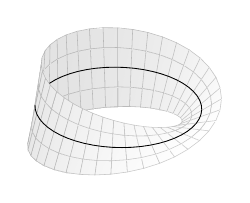
\begin{tikzpicture}[scale=0.5]
\begin{axis}[hide axis, view={40}{45}]
\addplot3 [surf, shader=faceted interp, point meta=x, colormap={slategraywhite}{rgb=(0.89,0.89,0.89) rgb=(1,1,1)},
samples=40, samples y=5, domain=0:360, y domain=-0.5:0.5]
({(1+0.5*y*cos(x/2)))*cos(x)}, {(1+0.5*y*cos(x/2)))*sin(x)}, {0.5*y*sin(x/2)});
\addplot3 [samples=50, domain=-142:184.5, samples y=0, semithick]
({cos(x)}, {sin(x)}, {0});
\end{axis}
\end{tikzpicture}
\end{center}

\vspace{-0.6cm}

It looks locally like the finite cylinder $S^1\times [0,1]$, which we can picture as the circle $S^1$ (the thicker
line in figure) with the finite interval $[0,1]$ attached to each of its points in a ``smooth'' way. The Möbious
strip has a ``twist'', which makes it globally different from the cylinder.

\bd [Topological Bundles]
A \textbf{topological bundle} (of topological manifolds) is a triple $(E,\pi,M)$ where $E$ and $M$ are topological
manifolds called the \emph{total space} and the \emph{base space} respectively, and $\pi$ is a continuous, surjective
map $\pi\cl E \to M$ called the \emph{projection map}.
\ed

We will often denote the bundle $(E,\pi,M)$ by $E\xrightarrow{\,\pi\,}M$.

\bd [Fiber]
Let $E\xrightarrow{\,\pi\,}M$ be a bundle and let $p\in M$. Then, $F_p \coloneqq \preim_\pi(\{p\})$ is called the
\textbf{fiber} at the point $p$.
\ed

Intuitively, the fiber at the point $p\in M$ is a set of points in $E$ (represented below as a line) attached to the
point $p$. The projection map sends all the points in the fiber $F_p$ to the point $p$.

\vspace{10pt}

\begin{figure}[H]
\centering
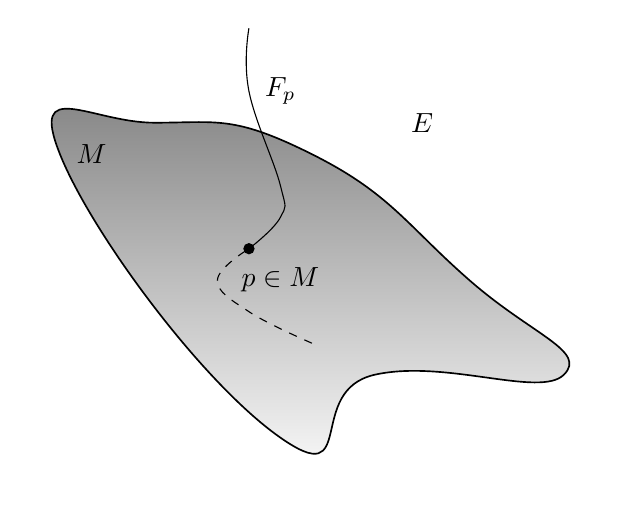
\begin{tikzpicture}[scale=0.8]
\draw[top color=gray,bottom color=white,semithick] plot[smooth cycle, tension=.9] coordinates {(-3,1.5)(-1.5,2)
(1,1.5) (3.5,-0.5) (5,-2) (2,-2) (0.5,-3)};
\node (v1) at (0,0) {};
\draw[dashed] plot[smooth, tension=.7] coordinates {(1,-1.5) (0,-1) (-0.5,-0.5) (v1)};
\draw plot[smooth, tension=.7] coordinates {(v1) (0.5,0.5) (0.5,1) (0,2.5) (0,3.5)};
\draw[fill=black] (v1) circle (0.08);
\node at (0.5,2.5) {$F_p$};
\node at (2.75,2) {$E$};
\node at (0.5,-0.5) {$p \in M$};
\node at (-2.5,1.5) {$M$};
\end{tikzpicture}
\end{figure}

\be
A trivial example of a bundle is the \emph{product bundle}. Let $M$ and $N$ be manifolds. Then, the triple $(M\times
N,\pi,M)$, where:
\bi{rrCl}
\pi \cl & M\times N & \to & M\\ & (p,q) & \mapsto & p
\ei

is a bundle since (one can easily check) $\pi$ is a continuous and surjective map. Similarly, $(M\times N,\pi,N)$
with the appropriate $\pi$, is also a bundle.
\ee

\be
In a bundle, different points of the base manifold may have (topologically) different fibers. For example, consider
the bundle $E\xrightarrow{\,\pi\,}\R$ where:
\bse
F_p \coloneqq \mathrm{preim}_\pi(\{p\}) \cong_\mathrm{top} \left\{ \ba{ll} S^1 &\t{if }p<0\\ \{p\} & \t{if }p=0\\ {}
[0,1] & \t{if } p>0 \ea \right.
\ese
\ee

\bd [Fiber Bundle]
Let $E\xrightarrow{\,\pi\,}M$ be a bundle and let $F$ be a manifold. Then, $E\xrightarrow{\,\pi\,}M$ is called a
\textbf{fiber bundle}, with (typical) fiber $F$, if:
\bse
\forall \, p \in M : \mathrm{preim}_\pi(\{p\}) \cong_\mathrm{top} F
\ese
\ed

A fiber bundle is often represented diagrammatically as: \v
\bse
\begin{tikzcd}
F\ar[r] & E \ar[d,"\pi"]\\ & M
\end{tikzcd}
\ese

\v

Let's provide some examples.

\be
The bundle $M\times N\xrightarrow{\,\pi\,}M$ is a fiber bundle with fiber $F \coloneqq N$.
\ee

\be
The Möbious strip is a fiber bundle $E\xrightarrow{\,\pi\,}S^1$, with fiber $F \coloneqq [0,1]$, where $E\neq
S^1\times[0,1]$, i.e.\ the Möbious strip is not a product bundle.
\ee

\be
A $\C$-line bundle over $M$ is the fiber bundle $(E,\pi,M)$ with fiber $\C$. Note that the product bundle $(M\times
\C,\pi,M)$ is a $\C$-line bundle over $M$, but a $\C$-line bundle over $M$ need not be a product bundle.
\ee

Now, let's move on providing the definition of a ``section''.

\bd [Section]
Let $E\xrightarrow{\,\pi\,}M$ be a bundle. A map $\s\cl M \to E$ is called a \textbf{section} of the bundle if
$\pi \circ \s = \id_M$.
\ed

Intuitively, a section is a map $\s$ which sends each point $p\in M$ to \emph{some} point $\s(p)$ in its fiber $F_p$,
so that the projection map $\pi$ takes $\s(p) \in F_p\se E$ back to the point $p\in M$.

\vspace{25pt}

\begin{figure}[H]
\centering
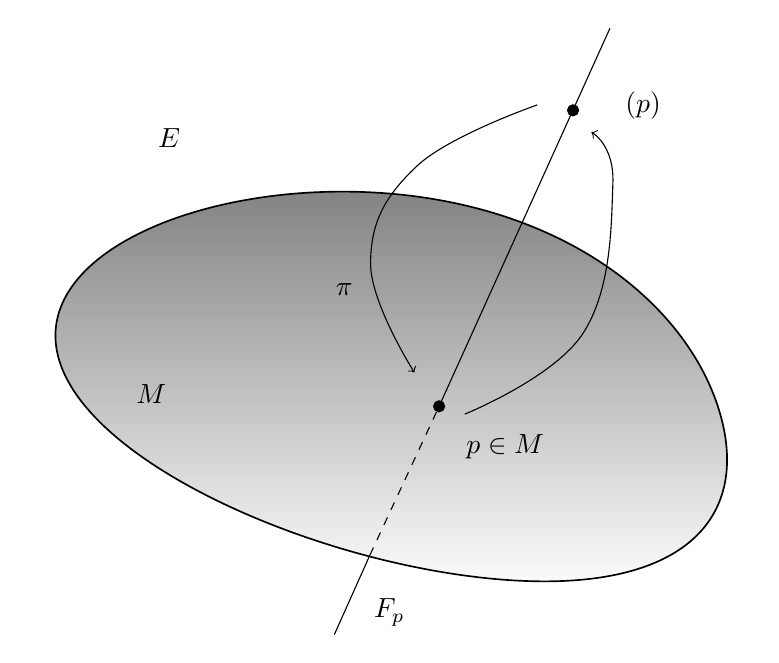
\begin{tikzpicture}[scale=1.4]
\draw[top color=gray,bottom color=white,semithick] plot[smooth cycle, tension=.99] coordinates {(-2.5,0) (0.5,1.5)
(3.5,-0.5) (1.5,-2)};
\draw (0,-2.5) -- (0.3224,-1.7792);
\draw[dashed] (0.3224,-1.7792) -- (0.9501,-0.4298);
\draw (0.9501,-0.4298)-- (2.5,3);
\node at (0.5,-2.3) {$F_p$};
\node at (1.55,-0.8) {$p \in M$};
\draw[fill=black] (0.9501,-0.4298) circle (0.05);
\draw [->] plot[smooth, tension=.7] coordinates {(1.1834,-0.5006) (2.2576,0.2354) (2.5265,1.5914) (2.3316,2.0564)};
\draw [->] plot[smooth, tension=.7] coordinates {(1.8399,2.3042) (0.7458,1.7472) (0.3281,0.872) (0.7259,-0.1226)};
\node at (0.09,0.6333) {$\pi$};
\node at (1.8,0.2) {$\s$};
\node at (-1.6612,-0.3216) {$M$};
\draw [fill=black] (2.1651,2.2555) circle (0.05);
\node at (2.8,2.3) {$\s(p)$};
\node at (-1.5,2) {$E$};
\end{tikzpicture}
\end{figure}

\vspace{10pt}

\be
Let $(M\times F,\pi,M)$ be a product bundle. Then, a section of this bundle is a map:
\bi{rrCl}
\s \cl & M & \to & M\times F\\ & p & \mapsto & (p,s(p))
\ei

where $s\cl M \to F$ is any map.
\ee

\bd [Sub-Bundle]
A \textbf{sub-bundle} of a bundle $(E,\pi,M)$ is a triple $(E',\pi',M')$ where $E'\se E$ and $M'\se M$ are submanifolds
and $\pi' \coloneqq \pi|_{E'}$.
\ed

\bd [Restricted Bundle]
Let $(E,\pi,M)$ be a bundle and let $N\se M$ be a submanifold. The \textbf{restricted bundle} (to $N$) is the triple
$(E,\pi',N)$ where:
\bse
\pi' \coloneqq \pi|_{\mathrm{preim}_\pi(N)}
\ese
\ed

\bd [Bundle Morphism]
Let $E\xrightarrow{\,\pi\,}M$ and $E'\xrightarrow{\,\pi'\,}M'$ be bundles and let $u\cl E\to E'$ and $v\cl M\to M'$
be maps. Then $(u,v)$ is called a \textbf{bundle morphism} if the following diagram commutes: \v
\bse
\begin{tikzcd}
E \ar[r,"u"] \ar[d,"\pi"]& E' \ar[d,"\pi'"]\\ M \ar[r,"v"]& M'
\end{tikzcd}
\ese

i.e.\ if $\pi'\circ u = v \circ \pi$.
\ed

\v

If $(u,v)$ and $(u,v')$ are both bundle morphisms, then $v=v'$. That is, given $u$, if there exists $v$ such that $
(u,v)$ is a bundle morphism, then $v$ is unique.

\bd [Isomorphic Bundles]
Two bundles $E\xrightarrow{\,\pi\,}M$ and $E'\xrightarrow{\,\pi'\,}M'$ are said to be \textbf{isomorphic (as bundles)}
if there exist bundle morphisms $(u,v)$ and $(u^{-1},v^{-1})$ satisfying: \v
\bse
\begin{tikzcd}
E \ar[rr,shift left,"u"] \ar[dd,"\pi"']&& E' \ar[ll,shift left,"u^{-1}"]\ar[dd,"\pi'"]\\
&&\\
M \ar[rr,shift left,"v"]&& M' \ar[ll,shift left,"v^{-1}"]
\end{tikzcd}
\ese

\v

Such a $(u,v)$ is called a \emph{bundle isomorphism} and we write
$E\xrightarrow{\, \pi\,}M \cong_{\mathrm{bdl}} E'\xrightarrow{\,\pi'\,}M'$.
\ed

Bundle isomorphisms are the structure-preserving maps for bundles. \v

Let's give some more definitions.

\bd [Locally Isomorphic Bundles]
A bundle $E\xrightarrow{\,\pi\,}M$ is said to be \textbf{locally isomorphic (as a bundle)} to a bundle
$E'\xrightarrow{\,\pi'\,}M'$ if for all $p\in M$ there exists a neighbourhood $U(p)$ such that the restricted bundle:
\bse
\mathrm{preim}_\pi(U(p))\xrightarrow{\,\pi|_{\mathrm{preim}_\pi(U(p))}\,}U(p)
\ese

\v

is isomorphic to the bundle $E'\xrightarrow{\,\pi'\,}M'$.
\ed

\bd [Trivial / Locally Trivial Bundle]
A bundle $E\xrightarrow{\,\pi\,}M$ is said to be:
\ben
\item[i)] \textbf{Trivial} if it is isomorphic to a product bundle.
\item[ii)] \textbf{Locally trivial} if it is locally isomorphic to a product bundle.
\een
\ed

\be
The cylinder $C$ is trivial as a bundle, and hence, also locally trivial.
\ee

\be
The Möbious strip is not trivial but it is locally trivial.
\ee

From now on, we will mostly consider locally trivial bundles. \v

In quantum mechanics, what is usually called a ``wave function'' is not a function at all, but rather a section of a
$\C$-line bundle over physical space. However, if we assume that the $\C$-line bundle under consideration is locally
trivial, then each section of the bundle can be represented (locally) by a map from the base space to the total space
and hence, it is appropriate to use the term ``wave \emph{function}''.

\bd [Pull-Back Bundle]
Let $E\xrightarrow{\,\pi\, }M$ be a bundle and let $f\cl M'\to M$ be a map from some manifold $M'$. The
\textbf{pull-back bundle of} $E\xrightarrow{\,\pi\, }M$ \emph{induced by} $f$ is defined as $E'\xrightarrow{\,\pi'\,}M'$,
where:
\bse
E' \coloneqq \{(m',e)\in M'\times E \mid f(m')=\pi(e)\}
\ese

and $\pi' (m',e) \coloneqq m'$.
\ed

If $E'\xrightarrow{\,\pi'\,}M'$ is the pull-back bundle of $E\xrightarrow{\,\pi\, }M$ induced by $f$, then one can
easily construct a bundle morphism by defining:
\bi{rcCl}
u \cl & E' & \to & E\\ & (m',e) & \mapsto & e
\ei

This corresponds to the diagram: \v
\bse
\begin{tikzcd}
E' \ar[d,"\pi'"] \ar[r,"u"] & E\ar[d,"\pi"]\\
M' \ar[r,"f"]& M
\end{tikzcd}
\ese

\v

Sections on a bundle pull back to the pull-back bundle. Indeed, let $E'\xrightarrow{\,\pi'\,}M'$ be the pull-back
bundle of $E\xrightarrow{\,\pi\, }M$ induced by $f$. \v

\bse
\begin{tikzcd}
E' \ar[dd,shift left,"\pi'"] && E\ar[dd,shift left,"\pi"]\\
&&\\
M' \ar[uurr,"\s\circ f"]\ar[uu,shift left,"\s'"]\ar[rr,"f"]&& M\ar[uu,shift left,"\s"]
\end{tikzcd}
\ese

\v

If $\s$ is a section of $E\xrightarrow{\,\pi\, }M$, then $\s \circ f$ determines a map from $M'$ to $E$ which sends
each $m'\in M'$ to $\s(f(m')) \in E$. However, since $\s$ is a section, we have:
\bse
\pi(\s(f(m'))= (\pi \circ \s \circ f)(m') = (\id_M\circ f)(m') = f(m')
\ese

and hence, $(m',(\s \circ f)(m'))\in E'$ by definition of $E'$. Moreover:
\bse
\pi' (m',(\s \circ f)(m')) = m'
\ese

and hence, the map:
\bi{rcCl}
\s' \cl & M' & \to & E'\\ & m' & \mapsto & (m',(\s \circ f)(m'))
\ei

satisfies $\pi'\circ\s'=\id_{M'}$ and it is thus a section on the pull-back bundle $E'\xrightarrow{\,\pi'\,}M'$.

\subsection{Tangent Bundle}

The reason of introducing the concept of a topological bundle, is because we need it in order to construct the so
called ``tangent bundle''. \v

As we said before, we want to define a vector field on a manifold $M$ as a ``smooth'' map that assigns to each $p\in
M$ a tangent vector in $T_p M$. The idea was to merge all the tangent spaces into a unique set and equip it with a
smooth structure, so that we can then define a vector field as a smooth map between smooth manifolds. We can do that
through the tangent bundle.

\bd [Tangent Bundle]
Given a smooth manifold $M$, the \textbf{tangent bundle} of $M$ is the disjoint union of all the tangent spaces to
$M$, i.e.\ :
\bse
TM \coloneqq \dot{\bigcup}_{p\in M}T_p M
\ese

equipped with the canonical projection map:
\bi{rrCl}
\pi \cl & TM & \to & M\\ & X_{\gamma,p} & \mapsto & p
\ei

where $p$ is the unique $p\in M$ such that $X_{\gamma,p} \in T_p M$.
\ed

In other word the projection map, takes a vector from $TM$ and spits out the point that it belongs $\pi(X_{\gamma,p})
= p$. \v

Since $TM$ is simpy a set (and not a smooth manifold), up to here what we have is a set bundle. In order for this set
bundle to turn to a topological bundle as we defined it previously, we need to equip $TM$ with the structure of a
smooth manifold. We can achieve this by constructing a smooth atlas for $TM$ from a smooth atlas on $M$, as follows. \v

Let $\mathscr{A}_M$ be a smooth atlas on $M$ and let $(U,x)\in \mathscr{A}_M$. If $X_{\gamma,p} \in \preim_\pi(U)\se
TM$, then $X_{\gamma,p} \in T_{\pi(X_{\gamma,p})}M$, by definition of $\pi$. Moreover, since $\pi(X_{\gamma,p}) = p
\in U$, we can expand $X_{\gamma,p}$ in terms of the basis induced by the chart $(U,x)$:
\bse
X_{\gamma,p} = X^a \tvb{x}{a}{p} = X^a \tvb{x}{a}{\pi(X_{\gamma,p})}
\ese

\v

where $X^1,\ldots,X^{\dim M}\in \R$. We can then define the map:
\bi{rrCl}
\xi \cl & \preim_\pi(U) & \to & x(U) \times \R^{\dim M} \cong_{\mathrm{set}}\R^{2\dim M}\\[5pt]
& X_{\gamma,p} & \mapsto & (x(\pi(X_{\gamma,p})),X^1,\ldots,X^{\dim M})
\ei

Assuming that $TM$ is equipped with a suitable topology, for instance the initial topology (i.e.\ the coarsest
topology on $TM$ that makes $\pi$ continuous), we claim that the pair $(\preim_\pi(U),\xi)$ is a chart on $TM$ and:
\bse
\mathscr{A}_{TM} \coloneqq \{(\preim_\pi(U),\xi)\mid (U,x) \in \mathscr{A}_M\}
\ese

\v

is a smooth atlas on $TM$. Note that, from its definition, it is clear that $\xi$ is a bijection. We will not show
that $(\preim_\pi(U),\xi)$ is a chart here, but we will show that $\mathscr{A}_{TM}$ is a smooth atlas.

\bt[]
Any two charts $(\preim_\pi(U),\xi), (\preim_\pi(\widetilde U),\widetilde \xi)\in\mathscr{A}_{TM}$ are
$\mathcal{C}^\infty$-compatible.
\et

\bq
Let $(U,x)$ and $(\widetilde U,\widetilde x)$ be the two charts on $M$ giving rise to $(\preim_\pi(U),\xi)$ and $
(\preim_\pi(\widetilde U),\widetilde \xi)$, respectively. We need to show that the map:
\bse
\widetilde \xi \circ \xi^{-1} \cl x(U\cap \widetilde U)\times \R^{\dim M} \to \widetilde x(U\cap\widetilde U)\times
\R^{\dim M}
\ese

is smooth, as a map between open subsets of $\R^{2\dim M}$. Recall that such a map is smooth if, and only if, it is
smooth componentwise. On the first $\dim M$ components, $\widetilde \xi \circ \xi^{-1} $ acts as:
\bi{rrCl}
\widetilde x \circ x^{-1} \cl & x(U\cap \widetilde U)& \to &\widetilde x(U\cap\widetilde U)\\
& x(p) & \mapsto & \widetilde x(p)
\ei

while on the remaining $\dim M$ components it acts as the change of vector components we met previously, i.e.\ :
\bse
X^a \mapsto \widetilde X^a = \partial_b(y^a\circ x^{-1})(x(p))\, X^b
\ese

Hence, we have:
\bi{rrCl}
\widetilde \xi \circ \xi^{-1} \cl & x(U\cap \widetilde U)\times \R^{\dim M} &\to &\widetilde x(U\cap\widetilde U)
\times \R^{\dim M}\\[5pt]
& (x(\pi(X_{\gamma,p})),X^1,\ldots,X^{\dim M})& \mapsto & (\widetilde x(\pi(X_{\gamma,p})),\widetilde X^1,\ldots,
\widetilde X^{\dim M})
\ei

which is smooth in each component, and hence, smooth.
\eq

The tangent bundle of a smooth manifold $M$ is therefore itself a smooth manifold of dimension $2\dim M$, and the
projection $\pi\cl TM\to M$ is smooth with respect to this structure. \v

Now by using the smooth manifold $M$ as the base space, the smooth manifold $TM$ as the total space, and the smooth
projection $\pi$ we can define the topological tangent bundle as the triple:
\bse
TM \projmapto M
\ese

\v

Similarly, one can construct the \emph{cotangent bundle} $T^*M$ to $M$ by defining:
\bse
T^*M \coloneqq \dot{\bigcup}_{p\in M} T^*_pM
\ese

and going through the above again, using the dual basis $\{(\d x^a)_p\}$ instead of $\{\tvb{x}{a}{p}\}$.

\subsection{Vector, Covector \& Tensor Fields}

Now that we have defined the tangent and cotangent bundles, we are ready to define fields.

\bd [Vector Field]
Let $M$ be a smooth manifold, and let $TM\xrightarrow{\,\pi\,}M$ be its tangent bundle. A \textbf{vector field} $X$ on
$M$ is a smooth section of the tangent bundle, i.e.\ a smooth map $X \cl M \to TM$ such that $\pi \circ X = \id_M$.
\bse
\begin{tikzcd}
TM \ar[dd,shift left,"\pi"] \\
\\
M \ar[uu,shift left,"X"]
\end{tikzcd}
\ese
\ed

\v

This might seem as an abuse of notation since we already use the symbol ``$X$'' to denote the tangent vectors
$X_{\gamma, p}$. However, there is a good reason for that since the two are very closely related, as we will see
right now. \v

We have already defined a smooth curve on a manifold M as a smooth map $\gamma\cl \R \to M$, where $\R$ is understood
as a $1$-dimensional manifold. We will now introduce the concept of the integral curve.

\bd [Integral Curve]
Let $M$ be a smooth manifold and let $X$ be a vector field on $M$. An \textbf{integral curve} of $X$ is smooth curve
$\gamma\cl(-\varepsilon,\varepsilon)\to M$, with $\varepsilon > 0$, such that:
\bse
\forall \, \lambda \in (-\varepsilon,\varepsilon) : \ X_{\gamma,\gamma(\lambda)} = X(\gamma(\lambda))
\ese
\ed

It follows from the local existence and uniqueness of solutions to ordinary differential equations that, given any
vector field $X$ and any point $p\in M$, there exist $\varepsilon >0$ and a smooth curve $\gamma\cl (-\varepsilon,
\varepsilon) \to M$ with $\gamma(0)=p$ which is an integral curve of $X$. \v

Moreover, integral curves are locally unique. By this we mean that if $\gamma_1$ and $\gamma_2$ are both integral
curves of $Y$ through $p$, i.e.\ $\gamma_1(0)=\gamma_2(0) = p$, then $\gamma_1=\gamma_2$ on the intersection of their
domains of definition.

\bd [Complete Vector Field]
A vector field is called \textbf{complete} if given an integral curve $\gamma\cl(-\varepsilon,\varepsilon)\to M$, the
domain of the integral curve $(-\varepsilon,\varepsilon)$ can be extended to $\R$ and still have:
\bse
\forall \, \lambda \in \R : \ X_{\gamma,\gamma(\lambda)} = X(\gamma(\lambda))
\ese
\ed

We have the following theorem.
\bt[]
On a compact manifold, every vector field is complete.
\et

Since we are only dealing with compact manifolds, we can draw the following conclusion. Every (complete) vector field
$X$ can act on a point $p$ of a manifold $M$ and produce the corresponding vector $X_{\gamma, p}$ in the sense that:
\bse
X(p) = X_{\gamma, p}
\ese

\v

and this is the reason why ``$X$'' and $X_{\gamma, p}$ are closely related. \v

From now on, we will drop the curve $\gamma$ from the notation of the vectors $X_{\gamma, p}$ and we will simply
write a vector as $X_p$. We do that for two reason: first in order to reduce the complexity of the equations
(although one has to remember that there is a curve $\gamma$ associated to every $X_p$) and second in order to have a
consistency with the way we denote covectors (i.e.\ $\omega_p$) where we do not denote the curve $\gamma$. Hence, from
now on the notation that we will be using is:
\bse
X(p) = X_p \implies X(p) f = X_p f
\ese

where $X$ is a vector field and when acted on a point $p$ produces the corresponding vector $X_p$. (From time to
time, when we will need to apply the definition of a vector, we will remind ourselves that $X_p$ actually means
$X_{\gamma, p}$ so we are not confused from the $\gamma$ in the definition). \v

As a final note, we also showed that a vector $X_p$ can be expressed in the coordinate induced basis as:
\bse
X_{p} = X^a \tvb{x}{a}{p}
\ese

Similarly for a vector field $X$ we will be writing:
\bse
X = X^a \cibasis{x^a}
\ese

where now $X^a$ are functions with $X^a(p)$ equal to $X^a$ from the vector equation i.e.\ :
\bse
X(p) = X^a(p) \tvb{x}{a}{p} = X^a \tvb{x}{a}{p} = X_p
\ese

In other words, this is more of a notation and not really a basis of vector fields $X$, since $\cibasis{x^a}$ must be
understood locally and not globally (more on that later).

\bd [$\Gamma(TM)$]
We denote the set of all vector fields on $M$ by $\Gamma(TM)$, i.e.\ :
\bse
\Gamma(TM) \coloneqq \{X \cl M \to TM \mid X \text{ is smooth and }\pi\circ X =\id_M\}
\ese
\ed

This is, in fact, the standard notation for the set of all sections on a bundle. \v

An equivalent definition is that a vector field $X$ on $M$ is a derivation on the algebra $\mathcal{C}^\infty(M)$, i.e.\
an $\R$-linear map: An equivalent definition is that a vector field $X$ on $M$ is a derivation on the algebra
$\mathcal{C}^\infty(M)$, i.e.\ an $\R$-linear map:
\bse
X \cl \mathcal{C}^\infty(M) \xrightarrow{\sim} \mathcal{C}^\infty(M)
\ese

\v

satisfying the Leibniz rule (with respect to pointwise multiplication on $\mathcal{C}^\infty(M)$):
\bse
X (fg) = g\, X(f) + f \, X(g)
\ese

This definition is better suited for some purposes, and later on we will switch from one to the other without making
any notational distinction between them. It also implies that a field $X$ instead of acting on a point $p$ of the
manifold, it can act directly to a function $f$ (and then evaluate at point $p$):
\bse
(Xf)(p) = X(p) f = X_p f
\ese

We can equip the set $\Gamma(TM)$ with the following operations. The first is our, by now familiar, pointwise addition:
\bi{rrCl}
\oplus \cl & \Gamma(TM) \times \Gamma(TM) & \to & \Gamma(TM)\\ & (X,Y) & \mapsto & X \oplus Y
\ei

where:
\bi{rrCl}
X \oplus Y \cl & M & \to & \Gamma(TM)\\ & p & \mapsto & (X \oplus Y)(p) \coloneqq X(p) + Y(p) = X_p + Y_p
\ei

Note that the $+$ on the right hand side above is the addition in $T_p M$. \v

More interestingly, we can define a multiplication operation not by a simple number (i.e.\ an element of $\R$) but with
a whole function (i.e.\ an element of $ \mathcal{C}^\infty(M)$) as follows:
\bi{rrCl}
\odot \cl & \mathcal{C}^\infty(M) \times \Gamma(TM) & \to & \Gamma(TM)\\ & (f,X) & \mapsto & f \odot X
\ei

where:
\bi{rrCl}
f \odot X \cl & M & \to & \Gamma(TM)\\ & p & \mapsto & (f\odot X)(p) \coloneqq f(p) X(p) = f(p) X_p
\ei

Note that since $f\in \mathcal{C}^\infty(M)$, we have $f(p)\in \R$ and hence, the multiplication above is the scalar
multiplication on $T_p M$. \v

Of course, we could have defined $\odot$ simply as pointwise \emph{global} scaling, using the reals $\R$ instead of
the real functions $\mathcal{C}^\infty(M)$. Then, since $(\R,+,\cdot)$ is an algebraic field, we would then have the
obvious $\R$-vector space structure on $\Gamma(TM)$, that we will also be using when needed. Let us make two comment
regarding this $\R$-vector space:
\bit
\item In the case of a function instead of a number, a function $f$ acts on the whole manifold $M$ (it assigns a
value $f(p)$ on every point $p$ of the manifold) and thus we are able to assign different values to different points.
In the case of $\R$-vector space we can only assign the same value to every point (i.e.\ having a constant vector field).
\item A basis for this corresponding $\R$-vector space is necessarily uncountably infinite, and hence, it does not
provide a very useful decomposition for our vector fields. On the other hand the operation $\odot$ allows for
\emph{local} scaling, i.e.\ we can scale a vector field by a different value at each point, and a much more useful
decomposition of vector fields.
\eit

The question now is, mathematically speaking, what exactly the triple $(\Gamma(TM),\oplus,\odot)$ is. Its nature of
course depends on what the triple $(\mathcal{C}^\infty(M),+,\cdot)$ is. Let's recall that the triple $
(\mathcal{C}^\infty(M),+,\cdot)$ can be viewed in two different ways:
\bit
\item $(\mathcal{C}^\infty(M),+,\cdot)$, where $\cdot$ is scalar multiplication (by a real number), is an
$\R$-vector space.
\item $(\mathcal{C}^\infty(M),+,\bullet)$, where $\bullet$ is pointwise multiplication of maps, is a commutative,
unital ring, but not a division ring since not every function has an inverse at every point (i.e.\ at all points that a
function is zero, we cannot define an inverse since we would divide by zero).
\eit

The first view is of no use since if the triple is seen as a vector space over the real numbers, there is nothing
else we can do. However, if we consider the second view, i.e.\ the triple $(\mathcal{C}^\infty(M),+,\bullet)$, where
$\bullet$ is pointwise function multiplication as a ring, then the triple $(\Gamma(TM),\oplus,\odot)$ built on top of
this ring satisfies:
\bit
\item $(\Gamma(TM),\oplus)$ is an abelian group, with $0\in \Gamma(TM)$ being the section that maps each $p\in M$
to the zero tangent vector in $T_p M$.
\item $\Gamma(TM)\sm\{0\}$ satisfies:
\ben[label=\roman*)]
\item $\forall \, f \in \mathcal{C}^\infty(M) : \forall \, X,Y \in \Gamma(TM) \sm\{0\}: f\odot(X\oplus Y)=(f\odot X)
\oplus (f\odot Y)$.
\item $\forall \, f,g \in \mathcal{C}^\infty(M) : \forall \, X \in \Gamma(TM)\sm\{0\}: (f+g)\odot X= (f \odot X)
\oplus (g \odot X)$.
\item $\forall \, f,g \in \mathcal{C}^\infty(M) : X \in \Gamma(TM)\sm\{0\} : (f\bullet g)\odot X= f \odot (g \odot X)$.
\item $\forall \, X \in \Gamma(TM) \sm\{0\} : 1 \odot X = X$, where $1\in \mathcal{C}^\infty(M)$ maps every $p\in
M$ to $1\in \R$.
\een
\eit

which are precisely the axioms for a vector space! hence, given that the triple $(\mathcal{C}^\infty(M),+,\bullet)$ is
a ring, that turns the triple $(\Gamma(TM),\oplus,\odot)$ to a $\mathcal{C}^\infty(M)$-module. \v

And this of course is of crucial importance since as we showed in previous chapters, if a ring $R$ is not a division
ring, then a $R$-module does not need to have a basis. And since as we already said $(\mathcal{C}^\infty(M),+, \bullet)$
is not a division ring, the vector fields as $\mathcal{C}^\infty(M)$-modules do not need to have a basis! And this is a
shame, since if they would have a basis (let's say $E_i$) we would be able to write a vector field $X$ as:
\bse
X = X^i E_i
\ese

where $X^i$ would be functions acting as components of the vector field! \v

Let us mention one final thing that will be useful later. Recall from the Lie algebra chapter in the notes, that a
Lie algebra over an algebraic field $K$ is a vector space over $K$ equipped with a Lie bracket $[-,-]$, i.e.\ a
$K$-bilinear, antisymmetric map which satisfies the Jacobi identity. \v

Considering $\Gamma(TM)$ as an infinite-dimensional $R$-vector space, for two vector fields $X,Y\in \Gamma(TM)$, we
can define their Lie bracket to be the commutator of the fields:
\bse
[X,Y] (f) \coloneqq X(Y(f))-Y(X(f))
\ese

for any $f\in \mathcal{C}^\infty(M)$. Now we can check that indeed $[X,Y]\in\Gamma(TM)$, and that the bracket is
$\R$-bilinear, antisymmetric and satisfies the Jacobi identity. Thus, $(\Gamma(TM),+,\cdot,[-,-])$ is an
infinite-dimensional Lie algebra over $\R$. (We usually suppress the $+$ and $\cdot$ when they are clear from the
context). \v

In a similar manner one can construct a covector field through the use of the cotangent bundle, and from there to
define the set of all covector fields $\Gamma(T^*M)$ and subsequently a triple $(\Gamma(T^*M), \oplus, \odot)$. \v

Finally, using $\Gamma(TM)$ and $\Gamma(T^*M)$ we can define a tensor field.

\bd [Tensor Field]
Let $M$ be a smooth manifold. A smooth \textbf{$(r,s)$ tensor field} $\tau$ on $M$ is a
$\mathcal{C}^\infty(M)$-multilinear map:
\bse
\tau \cl \underbrace{\Gamma(T^*M)\times \cdots \times \Gamma(T^*M)}_{r \text{ copies}} \times \underbrace{\Gamma(TM)
\times \cdots \times \Gamma(TM)}_{s \text{ copies}} \to \mathcal{C}^\infty(M)
\ese
\ed

The equivalence of this to the bundle definition is due to the pointwise nature of tensors. For instance, a covector
field $\omega\in \Gamma(T^*M)$ can act on a vector field $X\in\Gamma(TM)$ to yield a smooth function $\omega(X)
\in\mathcal{C}^\infty(M)$ which if it is evaluated at a specific point $p$ will yield a specific number:
\bse
(\omega(X))(p) \coloneqq \omega(p)(X(p)) = \omega_p (X_p)
\ese

\v

Then, we see that for any $f\in\mathcal{C}^\infty(M)$, we have:
\bse
(\omega(fX))(p) = \omega(p)(f(p)X(p)) = f(p)\omega(p)(X(p)) \eqqcolon (f\omega(X))(p)
\ese

\v

and hence, the map $\omega\cl \Gamma(TM)\xrightarrow{\sim}\mathcal{C}^\infty(M)$ is $\mathcal{C}^\infty(M)$-linear. \v

Similarly, the set $\Gamma(T^r_s M)$ of all $(r,s)$ smooth tensor fields on $M$ can be made into a $\mathcal{C}^\infty
(M)$-module, with module operations defined pointwise. \v

We can also define the tensor product of tensor fields:
\bi{rrCl}
\otimes \cl & \Gamma(T^p_qM) \times \Gamma(T^r_sM) & \to & \Gamma(T^{p+r}_{q+s}M)\\
&(\tau,\sigma) & \mapsto & \tau \otimes \sigma
\ei

analogously to what we had with tensors on a vector space, i.e.\ :
\bi{rl}
(\tau \otimes \sigma)(\omega^{(1)},\ldots,\omega^{(p)},\omega^{(p+1)},\ldots,\omega^{(p+r)},X^{(1)},&\ldots,X^{(q)},
X^{(q+1)},\ldots, X^{(q+s)})\\
\coloneqq \tau(\omega^{(1)},\ldots,\omega^{(p)}, X^{(1)},&\ldots,X^{(q)})\,\sigma(\omega^{(p+1)},\ldots,\omega^{(p+r)
},X^{(q+1)},\ldots, X^{(q+s)})
\ei

where the upper indices with the parenthesis count different vector and covector fields i.e.\ $\omega^{(i)}\in \Gamma
(T^*M)$ and $X^{(i)}\in \Gamma(TM)$. \v

Therefore, we can think of tensor fields on $M$ either as sections of some tensor bundle on $M$, that is, as maps
assigning to each $p\in M$ a tensor ($\R$-multilinear map) on the vector space $T_p M$, or as a $\mathcal{C}^\infty(M)
$-multilinear map as above. We will always try to pick the most useful or easier to understand, based on the context. \v

To summarize, fields are the generalization of the definitions of vectors, covectors and tensors at a specific point
$p$ of $M$, to every possible point $p$ of manifold $M$, hence, to the whole manifold $M$. In a similar way we can
generalize the concept of the gradient of $f$ at $p\in M$ in the gradient of $f$ at $M$.

\subsubsection*{Generalize (Gradient At A Point) To (Gradient Of The Manifold)}

Recall the definition of the gradient operator at a point $p\in M$. We can extend that definition to define the
($\R$-linear) operator:
\bi{rrCl}
\d \cl & \mathcal{C}^\infty(M) & \xrightarrow{\sim} & \Gamma(T^*M)\\ & f & \mapsto & \d f
\ei

where, of course, $\d f \cl p \mapsto \d_p f$. Alternatively, we can think of $\d f$ as the $\R$-linear map:
\bi{rrCl}
\d f \cl & \Gamma(TM) & \xrightarrow{\sim} & \mathcal{C}^\infty(M)\\ & X &\mapsto & \d f (X) = X(f)
\ei

Locally on some chart $(U,x)$ on $M$, the covector field $\d f$ can be expressed as:
\bse
\d f = \lambda_a\, \d x^a
\ese

for some smooth functions $\lambda_i\in\mathcal{C}^\infty(U)$. To determine what they are, we simply apply both sides
to the vector fields induced by the chart. We have:
\bse
\d f \biggl( \frac{\partial}{\partial x^b}\biggr) = \frac{\partial}{\partial x^b}(f) = \partial_bf
\ese

and:
\bse
\lambda_a\, \d x^a\biggl( \frac{\partial}{\partial x^b}\biggr) =\lambda_a\, \frac{\partial}{\partial x^b}(x^a) =
\lambda_a\,\delta^a_b = \lambda_b
\ese

\vspace{8pt}

Hence, the local expression of $\d f$ on $(U,x)$ is:
\bse
\d f = \partial_a f \, \d x^a
\ese

Note that the operator $\d$ satisfies the Leibniz rule:
\bse
\d (fg) = g\, \d f + f\, \d g
\ese

\subsubsection*{Generalize (Push-Forward \& Pull-Back At A Point) To (Push-Forward \& Pull-Back Of A Manifold)}

Finally, we want to generalize the concepts of push-forward and pull-back from a point to the whole manifold (a.k.a.\
from a vector/covector to a vector/covector field). For a good reason we will first start with the pull-back. \v

Recall that given a map $\phi\cl M \to N$ between smooth manifolds we defined the pull-back of $\phi$ at $p\in M$ as
the linear map:
\bi{rrCl}
(\phi^*)_p \cl & T^*_{\phi(p)}N & \xrightarrow{\sim} & T^*_pM\\
& \omega_{\phi(p)} & \mapsto & (\phi^*)_p(\omega_{\phi(p)})
\ei

where $(\phi^*)_p(\omega_{\phi(p)})$ is defined as:
\bi{rrCl}
(\phi^*)_p(\omega_{\phi(p)}) \cl & T_p M & \xrightarrow{\sim} & \R\\
& X_{\gamma,p} & \mapsto & (\phi^*)_p(\omega_{\phi(p)}) (X_{\gamma,p}) \coloneqq \omega_{\phi(p)}((\phi_*)_p
(X_{\gamma,p}))
\ei

Now we can simply extend the definition of a pull-back for a covector at point $p$ denoted $(\phi^*)_p$, to this of a
pull-back for a covector field on a manifold $M$ denoted $\phi^*$, by simpy acting with $(\phi^*)_p$ at every point
$p$ of the manifold $M$:
\bi{rrCl}
\phi^* \cl & \Gamma(T^*N )& \to & \Gamma(T^*M)\\ & \omega & \mapsto & \phi^*(\omega)
\ei

where $ \phi^*(\omega)$ evaluated at a point $p$ of $M$ is:
\bse
\phi^* (\omega)(p) \coloneqq (\phi^*)_p (\omega_{\phi(p)})
\ese

Hence, the pull-back of a covector field evaluated at point $p$ is equal to the pull-back of the covector
$\omega_{\phi(p)}$ generated by the covector field $\omega$ at point $\omega_{\phi(p)}$. \v

While the pull-back can be extended from covectros to covector fields without problems, the push-forward of a vector
cannot be generalized to the push-forward of a vector field unless the underlying map $\phi$ is a diffeomorphism
between the manifold $M$ and $N$. Let's see why. \v

Let's start again with the pull-back that we have already defined. Observe that the pull back of a covector field
includes the notion of the pull-back of a covector at a point $p$. Now, the map $\phi$, as a map, maps every single
point of its domain $M$ to a single point of its target $N$. Hence, the whole target $M$ is hit by the map, but the
whole target $N$ is not (recall that the part of $N$ that is hit by the map is called the image of $\phi$). This
means that in the case of a pull-back (after we have defined the tangent vectors in both $M$ and $N$) every single
point of the image of $\phi$ on $N$ will have a corresponding point back on $M$ hence, the definition of the pull-back
of a covector field will be well-defined. \v

On the other hand, in the case of a push forward we get two problems coming from the fact that, in general, the map
$\phi$ may not be neither surjective nor injective. First of all if the map $\phi$ is not surjective that means that
the image of $\phi$ is not equal to the entire domain $M$ ($\img_\phi(M) \neq N$), hence, from a vector field defined
on $M$ we will never be able to define a vector field on $N$ that lies outside the image of $\phi$. Moreover, if
$\phi$ is not injective, that means that distinct elements of the domain $M$ are mapped to the same element in the
target $N$ hence, it might be the case that the push-forward will create many different vectors for one given point
$p$ on $N$ which will make it ill-defined. \v

Of course, if the map $\phi$ is both surjective and injective, hence, bijective, hence, has an inverse, then none of
this problems exist any more, since then the case is similar to the case of pull-backs (both directions of the map
behave similarly). But recall that a bijection between topological spaces is called a ``homeomorphism'', and moreover
if the map is smooth (which in the case of smooth manifolds by definition always is) then the smooth ``homeomorphism''
is called a``diffeomorphism''. \v

So we ended up to our initial conclusion that the push-forward of a vector can be generalized to the push-forward of
a vector field only if the underlying map $\phi$ is a diffeomorphism between the manifold $M$ and $N$. Then we can
simply follow the same procedure as with the pull-back and define the push-forward of a vector field by simply acting
with the push-forward at every point $\phi(p)$ on the manifold $N$. \v

More specifically, recall that given a map $\phi\cl M \to N$ between smooth manifolds we defined the push-forward of
$\phi$ at $p\in M$ as the linear map:
\bi{rrCl}
(\phi_*)_p \cl & T_p M & \xrightarrow{\sim} & T_{\phi(p)}N\\ & X_{\gamma,p} & \mapsto & (\phi_*)_p(X_{\gamma,p})
\ei

where $(\phi_*)_p(X_{\gamma,p})$ is defined as:
\bi{rrCl}
(\phi_*)_p(X_{\gamma,p}) \cl & \mathcal{C}^\infty(N) & \xrightarrow{\sim} & \R\\
& f & \mapsto & (\phi_*)_p (X_{\gamma,p}) f \coloneqq X_{\gamma,p}(f \circ \phi)
\ei

Now we can simply extend the definition of a push-forward for a vector at point $p$ denoted $(\phi_*)_p$, to this of
a push-forward for a vector field on a manifold $M$ denoted $\phi*$, by simpy acting with the push-forward at every
point $p$ of the manifold $M$:
\bi{rrCl}
\phi_* \cl & \Gamma(TM) & \to & \Gamma(TN)\\ & X & \mapsto & \phi_*(X)
\ei

where $\phi_*(X)$ evaluated at a point $\phi(p)$ of $N$ is:
\bse
\phi_* (X) (\phi(p)) \coloneqq (\phi_*)_p (X_p)
\ese

Hence, the push-forward of a vector field evaluated at point $\phi(p)$ is equal to the push-forward of the vector
$X|_p$ generated by the vector field $X$ at point $p$. \v

Now let's move on another topic about ``differential forms''.

\section{Differential Forms}

\bd [Differential Form]
Let $M$ be a smooth manifold. A \textbf{(differential) $n$-form} on $M$ is a $(0,n)$ smooth tensor field $\omega$ which
is totally antisymmetric, i.e.\ :
\bse
\omega(X_1,\ldots,X_n) = \sgn(\pi)\, \omega(X_{\pi(1)},\ldots,X_{\pi(n)})
\ese

for any $\pi \in S_n$, with $X_i\in \Gamma(TM)$. We call $n$ the \emph{degree} of the form.
\ed

Alternatively, we can define a differential form as a smooth section of the appropriate bundle on $M$, i.e.\ as a map
assigning to each $p\in M$ an $n$-form on the vector space $T_p M$. \v

Of course, by definition, differential forms are nothing more but a very specific kind of tensors, hence, it's a
subset of the tensor space.

\be
The electromagnetic field strength $F$ is a differential $2$-form built from the electric and magnetic fields, which
are also taken to be forms. We will define these later in some detail.
\ee

\bd [$\Omega^n(M)$]
We denote by $\Omega^n(M)$ the set of all differential $n$-forms on $M$, which then becomes a $\mathcal{C}^\infty(M)
$-module by defining the addition and multiplication operations pointwise.
\ed

We have $\Omega^0(M)\equiv \mathcal{C}^\infty(M)$ since they are $(0,0)$ tensors a.k.a.\ functions and $\Omega^1(M)
\equiv \Gamma(T^0_1 M)\equiv\Gamma(T^*M)$ since they are $(0,1)$ tensors a.k.a.\ covectors. \v

We can specialise the pull-back of tensors to differential forms.

\bd [Pull-Back On Differential Forms]
Let $\phi\cl M \to N$ be a smooth map and let $\omega\in \Omega^n(N)$. Then we define the \textbf{pull-back} $\Phi^*
(\omega)\in \Omega^n(M)$ of $\omega$ as:
\bi{rrCl}
\Phi^*\cl & \Gamma(T^*N) &\to & \Gamma(T^*M)\\ & \omega & \mapsto & \Phi^*(\omega)
\ei

or equivalently:
\bi{rrCl}
\Phi^*\cl & \Omega^1(N) &\to & \Omega^1(M)\\ & \omega & \mapsto & \Phi^*(\omega)
\ei

where:
\bse
\Phi^*(\omega)(X^{(1)}\ldots,X^{(n)}) \coloneqq \omega \bigl( \phi_*(X^{(1)}),\ldots,\phi_*(X^{(n)}) \bigr)
\ese

\v

for vector fields $X^{(i)} \in \Gamma(TM)$ where $\phi_*(X^{(i)})$ is the push-forward of each vector field.
\ed

The map $\Phi^*\cl\Omega^n(N)\to\Omega^n(M)$ is $\R$-linear, and its action on $\Omega^0(M)$ is simply:
\bi{rrCl}
\Phi^*\cl & \Omega^0(M) & \to & \Omega^0(M)\\ &f &\mapsto &\Phi^*(f) \coloneqq f\circ \phi
\ei

This works for any smooth map $\phi$, and it leads to a slight modification of our mantra: \v

\begin{center}
\text{Vectors are pushed forward,}\\ \text{forms are pulled back.}
\end{center}

\v

The tensor product $\otimes$ does not interact well with forms, since the tensor product of two forms is not
necessarily a form (it might be, for example, a symmetric $(0,n)$ tensor which, be definition, is not a form). Hence,
we define the following.

\bd [Wedge Product]
Let $M$ be a smooth manifold. We define the \textbf{wedge} (or \emph{exterior}) \emph{product} of forms as the map:
\bi{rrCl}
\wedge \cl & \Omega^n(M) \times \Omega^m(M) & \to & \Omega^{n+m}(M)\\ & (\omega,\sigma) & \mapsto & \omega \wedge \sigma
\ei

where:
\bse
(\omega\wedge\sigma)(X_1,\ldots,X_{n+m}) \coloneqq \frac{1}{n!\,m!} \sum_{\pi \in S_{n+m}} \sgn(\pi) (\omega
\otimes \sigma)(X_{\pi(1)},\ldots,X_{\pi(n+m)})
\ese

\v

and $X_1,\ldots,X_{n+m}\in\Gamma(TM)$. By convention, for any $f,g\in \Omega^0(M)$ and $\omega\in \Omega^n(M)$, we set:
\bse
f\wedge g \coloneqq fg \qquad \text{and} \qquad f\wedge\omega=\omega\wedge f = f\omega
\ese
\ed

Let's see an example.

\be
Suppose that $\omega,\sigma\in\Omega^1(M)$. Then, for any $X,Y\in\Gamma(TM)$:
\bi{rCl}
(\omega\wedge\sigma)(X,Y) & = & (\omega\otimes\sigma)(X,Y) - (\omega\otimes\sigma)(Y,X)\\
& = & (\omega\otimes\sigma)(X,Y) - \omega(Y)\sigma(X)\\
& = & (\omega\otimes\sigma)(X,Y) - (\sigma \otimes \omega)(X,Y)\\
& = & (\omega\otimes\sigma -\sigma \otimes \omega)(X,Y)
\ei

Hence:
\bse
\omega\wedge\sigma = \omega\otimes\sigma - \sigma \otimes \omega.
\ese
\ee

\v

The wedge product is bilinear over $\mathcal{C}^\infty(M)$, that is:
\bse
(f\omega_1 +\omega_2)\wedge \sigma = f\, \omega_1\wedge\sigma+\omega_2\wedge\sigma
\ese

for all $f\in\mathcal{C}^\infty(M)$, $\omega_1,\omega_2\in\Omega^n(M)$ and $\sigma\in\Omega^m(M)$, and similarly for
the second argument. \v

If $(U,x)$ is a chart on $M$, then every $n$-form $\omega\in \Omega^n(U)$ can be expressed locally on $U$ as:
\bse
\omega = \omega_{a_1\cdots a_n} \, \d x^{a_1} \wedge \cdots \wedge \d x^{a_n}
\ese

where $\omega_{a_1\cdots a_n}\in \mathcal{C}^\infty(U)$ and $1\leq a_1 < \cdots < a_n \leq \dim M$. The $\d x^{a_i}$
appearing above are the covector fields ($1$-forms):
\bse
\d x^{a_i} \cl p\mapsto \d_px^{a_i}
\ese

\v

The pull-back distributes over the wedge product.

\bt[]
Let $\phi\cl M\to N$ be smooth, $\omega\in\Omega^n(N)$ and $\sigma\in\Omega^m(N)$. Then, we have:
\bse
\Phi^*(\omega\wedge\sigma) = \Phi^*(\omega)\wedge\Phi^*(\sigma)
\ese
\et

Let's prove this.

\bq
Let $p\in M$ and $X_1,\ldots,X_{n+m}\in T_p M$. Then we have:
\bi{rCl}
\IEEEeqnarraymulticol{3}{l}{\bigl( \Phi^*(\omega)\wedge\Phi^*(\sigma) \bigr) (p)(X_1,\ldots,X_{n+m}) }\\[5pt]
\qquad \qquad & = & \frac{1}{n!\,m!} \sum_{\pi \in S_{n+m}} \sgn(\pi) \bigl( \Phi^*(\omega)\otimes\Phi^*(\sigma)
\bigr)(p)(X_{\pi(1)},\ldots,X_{\pi(n+m)})\\[5pt]
& = & \frac{1}{n!\,m!} \sum_{\pi \in S_{n+m}} \sgn(\pi)\Phi^*(\omega)(p)(X_{\pi(1)},\ldots,X_{\pi(n)})\\[-10pt]
& & \hspace{3.9cm} \Phi^*(\sigma) (p)(X_{\pi(n+1)},\ldots,X_{\pi(n+m)})\\[5pt]
& = & \frac{1}{n!\,m!} \sum_{\pi \in S_{n+m}} \sgn(\pi)\omega(\phi(p))\bigl( \phi_*(X_{\pi(1)}),\ldots,\phi_*(X_{\pi
(n)})\bigr) \\[-10pt]
& & \hspace{4.4cm} \sigma(\phi(p))\bigl( \phi_*(X_{\pi(n+1)}),\ldots,\phi_*(X_{\pi(n+m)})\bigr)\\[5pt]
& = & \frac{1}{n!\,m!} \sum_{\pi \in S_{n+m}}\sgn(\pi) (\omega\otimes\sigma) (\phi(p)) \bigl( \phi_*(X_{\pi(1)}),
\ldots,\phi_*(X_{\pi(n+m)})\bigr)\\[5pt]
& = & (\omega\wedge\sigma) (\phi(p)) \bigl( \phi_*(X_1),\ldots,\phi_*(X_{n+m})\bigr)\\[5pt]
& = & \Phi^*(\omega\wedge\sigma) (p) ( X_1,\ldots,X_{n+m})
\ei

Since $p\in M$ was arbitrary, the statement follows.
\eq

\subsection{The Grassmann Algebra}

Note that the wedge product takes two differential forms and produces a differential form of a different type. It
would be much nicer to have a space which is closed under the action of $\wedge$. In fact, such a space exists and it
is called the Grassmann algebra of $M$.

\bd [Grassmann Algebra]
Let $M$ be a smooth manifold. Define the $\mathcal{C}^\infty(M)$-module:
\bse
\Gr(M)\equiv\Omega(M) \coloneqq \bigoplus_{n=0}^{\dim M} \Omega^n(M)
\ese

The \textbf{Grassmann algebra} on $M$ is the algebra $(\Omega(M),+,\cdot,\wedge)$, where:
\bse
\wedge\cl \Omega(M)\times\Omega(M)\to\Omega(M)
\ese

is the linear continuation of the previously defined $\wedge\cl\Omega^n(M)\times\Omega^m(M)\to\Omega^{n+m}(M)$.
\ed

Recall that the direct sum of modules has the Cartesian product of the modules as underlying set and module
operations defined componentwise. Also, note that by ``algebra'' here we really mean ``algebra over a module''.

\be
Let $\psi=\omega+\sigma$, where $\omega\in\Omega^1(M)$ and $\sigma\in\Omega^3(M)$. Of course, this ``+'' is neither
the addition on $\Omega^1(M)$ nor the one on $\Omega^3(M)$, but rather that on $\Omega(M)$ and, in fact,
$\psi\in\Omega(M)$. \v

Let $\varphi\in \Omega^n(M)$, for some $n$. Then:
\bse
\varphi\wedge\psi=\varphi\wedge(\omega+\sigma)= \varphi\wedge\omega+\varphi\wedge\sigma
\ese

where $\varphi\wedge\omega\in\Omega^{n+1}(M)$, $\varphi\wedge\sigma\in\Omega^{n+3}(M)$, and
$\varphi\wedge\psi\in\Omega(M)$.
\ee

\be
There is a lot of talk about \emph{Grassmann numbers}, particularly in supersymmetry. One often hears that these are
``numbers that do not commute, but anticommute''. Of course, objects cannot be commutative or anticommutative by
themselves. These qualifiers only apply to operations on the objects. In fact, the Grassmann numbers are just the
elements of a Grassmann algebra.
\ee

The following theorem is about the anticommutative behaviour of $\wedge$.

\bt[]
Let $\omega\in\Omega^n(M)$ and $\sigma\in\Omega^m(M)$. Then:
\bse
\omega\wedge\sigma=(-1)^{nm}\,\sigma\wedge\omega
\ese
\et

We say that $\wedge$ is \emph{graded commutative}, that is, it satisfies a version of anticommutativity which depends
on the degrees of the forms.

\bq
First note that if $\omega,\sigma\in\Omega^1(M)$, then:
\bse
\omega\wedge\sigma = \omega\otimes\sigma - \sigma \otimes \omega = \negmedspace {}- \sigma \wedge \omega
\ese

Recall that is $\omega\in\Omega^n(M)$ and $\sigma\in\Omega^m(M)$, then locally on a chart $(U,x)$ we can write:
\bi{C}
\omega = \omega_{a_1\cdots a_n}\d x^{a_1}\wedge \cdots \wedge \d x^{a_n} \\
\sigma = \sigma_{b_1\cdots b_m}\d x^{b_1}\wedge \cdots \wedge \d x^{b_m}
\ei

with $1\leq a_1 < \cdots < a_n \leq \dim M$ and similarly for the $b_i$. The coefficients $\omega_{a_1\cdots a_n}$
and $\sigma_{b_1\cdots b_m}$ are smooth functions in $\mathcal{C}^\infty(U)$. Since $\d x^{a_i},\d x^{b_j}\in
\Omega^1(M)$, we have:
\bi{rCl}
\omega\wedge\sigma & = & \omega_{a_1\cdots a_n}\sigma_{b_1\cdots b_m}\,\d x^{a_1}\wedge \cdots \wedge \d
x^{a_n}\wedge\d x^{b_1}\wedge \cdots \wedge \d x^{b_m}\\[5pt]
& = &(-1)^n\,\omega_{a_1\cdots a_n}\sigma_{b_1\cdots b_m}\,\d x^{b_1}\wedge\d x^{a_1}\wedge \cdots \wedge \d
x^{a_n}\wedge\d x^{b_2}\wedge \cdots \wedge \d x^{b_m}\\[5pt]
& = &(-1)^{2n}\,\omega_{a_1\cdots a_n}\sigma_{b_1\cdots b_m}\,\d x^{b_1}\wedge\d x^{b_2}\wedge\d x^{a_1}\wedge \cdots
\wedge \d x^{a_n}\wedge\d x^{b_3}\wedge \cdots \wedge \d x^{b_m}\\[5pt]
& \vdots &\\[5pt]
& = &(-1)^{nm}\,\omega_{a_1\cdots a_n}\sigma_{b_1\cdots b_m}\,\d x^{b_1}\wedge \cdots \wedge \d x^{b_m}\wedge\d
x^{a_1}\wedge \cdots \wedge \d x^{a_n}\\[5pt]
& = & (-1)^{nm} \, \sigma \wedge \omega
\ei

since we have swapped $1$-forms $nm$-many times.
\eq

We should stress that this is only true when $\omega$ and $\sigma$ are pure degree forms, rather than linear
combinations of forms of different degrees. Indeed, if $\varphi,\psi\in\Omega(M)$, a formula like:
\bse
\varphi\wedge\psi = \cdots \psi \wedge \varphi
\ese

does not make sense in principle, because the different parts of $\varphi$ and $\psi$ can have different commutation
behaviours.

\subsection{The Exterior Derivative}

Recall the ``extended'' definition of the gradient operator of a function $\d$ on the whole manifold $M$:
\bi{rrCl}
\d \cl & \mathcal{C}^\infty(M) & \xrightarrow{\sim} & \Gamma(T^*M)\\ & f & \mapsto & \d f
\ei

Since $\Omega^0(M)\equiv \mathcal{C}^\infty(M)$ and $\Omega^1(M)\equiv \Gamma(T^0_1 M)\equiv\Gamma(T^* M)$, we can also
understand this as an operator that takes in $0$-forms and outputs $1$-forms:
\bse
\d \cl \Omega^0(M)\xrightarrow{\sim}\Omega^1(M)
\ese

This can then be extended to an operator which acts on any $n$-form. For this definition, we need to remind ourselves
of the definition of commutator we gave in the algebra section of the notes. More precisely, if $M$ is a smooth
manifold and $X,Y\in\Gamma(TM)$ then the commutator (or Lie bracket) of $X$ and $Y$ is defined as:
\bi{rrCl}
[X,Y]\cl & \mathcal{C}^\infty(M) &\xrightarrow{\sim} &\mathcal{C}^\infty(M)\\
& f & \mapsto & [X,Y](f) \coloneqq X(Y(f))-Y(X(f))
\ei

where we are using the definition of vector fields as $\R$-linear maps $\mathcal{C}^\infty(M) \xrightarrow{\sim}
\mathcal{C}^\infty(M)$. \v

Using the commutator we can now extend the gradient as follows.

\bd [Exterior Derivative]
The \textbf{exterior derivative} on $M$ is the $\R$-linear operator:
\bi{rrCl}
\d\cl &\Omega^n(M)&\xrightarrow{\sim} &\Omega^{n+1}(M)\\ & \omega & \mapsto & \d \omega
\ei

with $\d \omega$ being defined as:
\bi{rCl}
\d \omega (X^{(1)},\ldots,X^{(n+1)}) & \coloneqq & \sum_{i=1}^{n+1} (-1)^{i+1}\, X^{(i)} \bigl(\omega(X^{(1)},
\ldots,\widehat{X^{(i)}},\ldots,X^{(n+1)})\bigr)\\[5pt]
& & {} \negmedspace + \sum_{i<j} (-1)^{i+j}\,\omega\bigl([X^{(i)},X^{(j)}],X^{(1)},\ldots,\widehat{X^{(i)}},\ldots,
\widehat{X^{(j)}},\ldots,X^{(n+1)}\bigr)
\ei

where $X^{(i)}\in \Gamma(TM)$ and the hat denotes omissions.
\ed

Note that the operator $\d$ is only well-defined when it acts on forms. In order to define a derivative operator on
general tensors we will need to add extra structure to our differentiable manifold. \v

By using the exterior derivative, the picture for $1$-forms extends to higher dimensions. For example, assuming
vanishing Lie brackets to simplify the picture, the exterior derivative of a $2$-form can be viewed as the “sum on
the boundary faces of the cube defined by its arguments”.

\fig{form}{1}

Before we move on let's see in practice how exterior derivatives works through an example.

\be
In the case $n=1$, the form $\d \omega\in\Omega^2(M)$ is given by:
\bse
\d \omega (X,Y) = X(\omega(Y))-Y(\omega(X))-\omega([X,Y])
\ese

Let us check that this is indeed a $2$-form, i.e.\ an antisymmetric, $\mathcal{C}^\infty(M)$-multilinear map:
\bse
\d\omega\cl \Gamma(TM)\times\Gamma(TM)\to\mathcal{C}^\infty(M)
\ese

By using the antisymmetry of the Lie bracket, we immediately get:
\bse
\d \omega(X,Y)= - \,\d\omega(Y,X)
\ese

Moreover, thanks to this identity, it suffices to check $\mathcal{C}^\infty(M)$-linearity in the first argument only.
Additivity is easily checked:
\bi{rCl}
\d\omega(X+Y,Z) & = & (X+Y)(\omega(Z))-Z(\omega(X+Y))-\omega([X+Y,Z])\\[5pt]
& = & X(\omega(Z))+Y(\omega(Z))-Z(\omega(X)+\omega(Y))-\omega([X,Z]+[Y,Z])\\[5pt]
& = & X(\omega(Z))+Y(\omega(Z))-Z(\omega(X))-Z(\omega(Y))-\omega([X,Z])-\omega([Y,Z])\\[5pt]
&=& \d\omega(X,Z) +\d\omega(Y,Z)
\ei

For $\mathcal{C}^\infty(M)$-scaling, first we calculate $[fX,Y]$. Let $g\in\mathcal{C}^\infty(M)$. Then:
\bi{rCl}
[fX,Y](g) &=& fX(Y(g)) -Y (fX(g))\\[5pt]
&=& fX(Y(g)) - fY(X(g)) -Y (f)X(g)\\[5pt]
&=& f(X(Y(g)) - Y(X(g))) -Y (f)X(g)\\[5pt]
&=& f[X,Y](g) -Y(f)X(g)\\[5pt]
&=& (f[X,Y] -Y(f)X)(g)
\ei

Therefore:
\bse
[fX,Y]=f[X,Y]-Y(f)X
\ese

Hence, we can calculate:
\bi{rCl}
\d\omega(fX,Y) & = & fX(\omega(Y))-Y(\omega(fX))-\omega([fX,Y])\\[5pt]
& = & fX(\omega(Y))-Y(f\omega(X))-\omega(f[X,Y]-Y(f)X)\\[5pt]
& = & fX(\omega(Y))-fY(\omega(X))-Y(f)\omega(X)-f\omega([X,Y])+\omega(Y(f)X)\\[5pt]
& = & fX(\omega(Y))-fY(\omega(X))-\cancel[gray]{Y(f)\omega(X)}-f\omega([X,Y])+\cancel[gray]{Y(f)\omega(X)}\\[5pt]
&=& f\,\d\omega(X,Y)
\ei

which is what we wanted.
\ee

The exterior derivative satisfies a graded version of the Leibniz rule with respect to the wedge product. This can be
formalized in a theorem.

\bt[]
Let $\omega\in\Omega^n(M)$ and $\sigma\in\Omega^m(M)$. Then:
\bse
\d(\omega\wedge\sigma)=\d\omega\wedge\sigma+(-1)^n\,\omega\wedge\d\sigma
\ese
\et

\bq
We will work in local coordinates. Let $(U,x)$ be a chart on $M$ and write:
\bi{C}
\omega = \omega_{a_1\cdots a_n}\d x^{a_1}\wedge \cdots \wedge \d x^{a_n} \eqqcolon \omega_A \d x^A\\[5pt]
\sigma = \sigma_{b_1\cdots b_m}\d x^{b_1}\wedge \cdots \wedge \d x^{b_m} \eqqcolon \sigma_B \d x^B
\ei

Locally, the exterior derivative operator $\d$ acts as:
\bse
\d \omega = \d \omega_A \wedge \d x^A
\ese

Hence:
\bi{rCl}
\d (\omega\wedge\sigma) & = & \d (\omega_A\sigma_B\, \d x^A\wedge \d x^B)\\[5pt]
& = & \d (\omega_A\sigma_B)\wedge\d x^A\wedge \d x^B\\[5pt]
& = & (\sigma_B \d \omega_A +\omega_A\d\sigma_B)\wedge\d x^A\wedge \d x^B\\[5pt]
& = & \sigma_B \d \omega_A\wedge\d x^A\wedge \d x^B+\omega_A\d\sigma_B \wedge\d x^A\wedge \d x^B\\[5pt]
& = & \sigma_B \d \omega_A\wedge\d x^A\wedge \d x^B+(-1)^n\omega_A\d x^A\wedge\d\sigma_B \wedge \d x^B\\[5pt]
& = & \sigma_B \d \omega\wedge \d x^B+(-1)^n\omega_A\d x^A\wedge\d\sigma\\[5pt]
& = & \d \omega\wedge \sigma+(-1)^n\, \omega\wedge\d\sigma
\ei

since we have ``anticommuted'' the $1$-form $\d\sigma_B$ through the $n$-form $\d x^A$, picking up $n$ minus signs in
the process.
\eq

An important property of the exterior derivative is the following.

\bt[]
Let $\phi\cl M\to N$ be smooth. For any $\omega\in\Omega^n(N)$, we have:
\bse
\Phi^*(\d \omega) = \d (\Phi^*(\omega))
\ese
\et

Informally, we can write this result as $\Phi^*\d=\d\Phi^*$, and say that the exterior derivative ``commutes'' with
the pull-back. \v

However, you should bear in mind that the two $\d$'s appearing in the statement are two different operators. On the
left hand side, it is $\d\cl\Omega^n(N)\to\Omega^{n+1}(N)$, while it is $\d\cl\Omega^n(M)\to\Omega^{n+1}(M)$ on the
right hand side. \v

Of course, we could also combine the operators $\d$ into a single operator acting on the Grassmann algebra on $M$:
\bse
\d \cl \Omega(M)\to\Omega(M)
\ese

by linear continuation.

\subsection{De Rham Cohomology}

\bd [Closed / Exact Forms]
Let $M$ be a smooth manifold and let $\omega \in \Omega^n(M)$. We say that $\omega$ is:
\bit
\item \textbf{Closed} if $\d \omega = 0$.
\item \textbf{Exact} if $\exists \, \sigma \in \Omega^{n-1}(M): \omega = \d \sigma$.
\eit
\ed

The question of whether every closed form is exact and vice versa, i.e.\ whether the implications:
\bse
(\d \omega =0) \Leftrightarrow (\exists \, \sigma : \omega =\d \sigma)
\ese

hold in general, belongs to the branch of mathematics called cohomology theory, to which we will now provide an
introduction. \v

The answer for the $\Leftarrow$ direction is affirmative thanks to the following theorem.

\bt[]
Let $M$ be a smooth manifold. The operator:
\bse
\d^2 \equiv \d \circ \d \cl \Omega^n(M) \to \Omega^{n+2}(M)
\ese

is identically zero, i.e.\ $\d^2=0$.
\et

\bq
This can be shown directly using the definition of $\d$. Here, we will instead show it by working in local
coordinates. \v

Recall that, locally on a chart $(U,x)$, we can write any form $\omega\in\Omega^n(M)$ as:
\bse
\omega = \omega_{a_1\cdots a_n}\d x^{a_1}\wedge \cdots \wedge \d x^{a_n}
\ese

Then, we have:
\bi{rCl}
\d \omega & = & \d \omega_{a_1\cdots a_n}\wedge\d x^{a_1}\wedge \cdots \wedge \d x^{a_n}\\[5pt]
& = & \partial_b \omega_{a_1\cdots a_n}\d x^b\wedge\d x^{a_1}\wedge \cdots \wedge \d x^{a_n}
\ei

and hence:
\bse
\d^2\omega = \partial_c\partial_b\omega_{a_1\cdots a_n}\d x^c\wedge\d x^b\wedge\d x^{a_1}\wedge \cdots \wedge \d x^{a_n}
\ese

\v

We can perform a little ``trick'' in the last equation and write it as twice the half expression:
\bse
\d^2\omega = \frac{1}{2} \partial_c\partial_b\omega_{a_1\cdots a_n}\d x^c\wedge\d x^b\wedge\d x^{a_1}\wedge \cdots
\wedge \d x^{a_n} + \frac{1}{2} \partial_c\partial_b\omega_{a_1\cdots a_n}\d x^c\wedge\d x^b\wedge\d x^{a_1}\wedge
\cdots \wedge \d x^{a_n}
\ese

Now we can inter-switch the $c$ and $b$ dummy indices in the second half part (we can do it since they are just dummy
indices) and we get:
\bse
\d^2\omega = \frac{1}{2} \partial_c\partial_b\omega_{a_1\cdots a_n}\d x^c\wedge\d x^b\wedge\d x^{a_1}\wedge \cdots
\wedge \d x^{a_n} + \frac{1}{2} \partial_b\partial_c\omega_{a_1\cdots a_n}\d x^b\wedge\d x^c\wedge\d x^{a_1}\wedge
\cdots \wedge \d x^{a_n}
\ese

Since $\d x^b\wedge\d x^c = - \, \d x^c\wedge\d x^b$, and moreover, by Schwarz's theorem, we have
$\partial_c\partial_b\omega_{a_1\cdots a_n} = \partial_b\partial_c\omega_{a_1\cdots a_n}$ we get:
\bse
\d^2\omega =\frac{1}{2} \partial_c\partial_b\omega_{a_1\cdots a_n}\d x^c\wedge\d x^b\wedge\d x^{a_1}\wedge \cdots
\wedge \d x^{a_n} - \frac{1}{2} \partial_c\partial_b\omega_{a_1\cdots a_n}\d x^c\wedge\d x^b\wedge\d x^{a_1}\wedge
\cdots \wedge \d x^{a_n}
\ese

Hence:
\bse
\d^2\omega = 0
\ese

Since this holds for any $\omega$, we have $\d^2=0$.
\eq

\bt[]
Every exact form is closed.
\et

We can extend the action of $\d$ to the zero vector space $0 \coloneqq \{0\}$ by mapping the zero in $0$ to the zero
function in $\Omega^0(M)$. In this way, we obtain the chain of $\R$-linear maps:
\bse
0 \xrightarrow{\ \d\ } \Omega^0(M)\xrightarrow{\ \d\ } \Omega^1(M)\xrightarrow{\ \d\ } \cdots \xrightarrow{\ \d\ }
\Omega^{n}(M)\xrightarrow{\ \d\ } \Omega^{n+1}(M)\xrightarrow{\ \d\ } \cdots \xrightarrow{\ \d\ } \Omega^{\dim M}(M)
\xrightarrow{\ \d\ } 0
\ese

where we now think of the spaces $\Omega^n(M)$ as $\R$-vector spaces. \v

Recall from linear algebra section in the notes that, given a linear map $\phi \cl V \to W$, one can define the
subspace of $V$:
\bse
\ker(\phi) \coloneqq \{v \in V \mid \phi(v)=0\}
\ese

\v

called the \emph{kernel} of $\phi$, and the subspace of $W$:
\bse
\im (\phi) \coloneqq \{\phi(v)\mid v \in V\}
\ese

called the \emph{image} of $\phi$. \v

Going back to our chain of maps, the equation $\d^2=0$ is equivalent to:
\bse
\im(\d \cl \Omega^n(M)\to\Omega^{n+1}(M)) \se \ker(\d \cl \Omega^{n+1}(M)\to\Omega^{n+2}(M))
\ese

for all $0\leq n \leq \dim M-2$. Moreover, we have:
\bi{rCl}
\omega \in \Omega^n(M) \text{ is closed } & \Leftrightarrow\ & \omega \in \ker(\d \cl \Omega^n(M)\to\Omega^{n+1}(M))\\
\omega \in \Omega^n(M) \text{ is exact } & \Leftrightarrow\ & \omega \in \im (\d \cl \Omega^{n-1}(M)\to\Omega^{n}(M))
\ei

The traditional notation for the spaces on the right hand side above is:
\bi{rCl}
Z^n & \coloneqq & \ker(\d \cl \Omega^n(M)\to\Omega^{n+1}(M))\\
B^n & \coloneqq & \im (\d \cl \Omega^{n-1}(M)\to\Omega^{n}(M))
\ei

so that $Z^n$ is the space of closed $n$-forms and $B^n$ is the space of exact $n$-forms. \v

Our original question can be restated as: does $Z^n=B^n$ for all $n$? We have already seen that $\d^2=0$ implies that
$B^n\se Z^n$ for all $n$ ($B^n$ is, in fact, a vector subspace of $Z^n$). Unfortunately the equality does not hold in
general, but we do have the following result.

\bt[Poincaré Lemma]
Let $M\se \R^d$ be a simply connected domain. Then:
\bse
Z^n = B^n \, , \qquad \forall \, n > 0
\ese
\et

In the cases where $Z^n\neq B^n$, we would like to quantify by how much the closed $n$-forms fail to be exact. The
answer is provided by the cohomology group.

\bd [de Rham Cohomology Group]
Let $M$ be a smooth manifold. The $n$-th \textbf{de Rham cohomology group} on $M$ is the quotient $\R$-vector space:
\bse
H^n(M) \coloneqq Z^n/B^n
\ese
\ed

You can think of the above quotient as $Z^n/\!\sim$, where $\sim$ is the equivalence relation:
\bse
\omega \sim \sigma\ :\Leftrightarrow\ \omega-\sigma \in B^n
\ese

The answer to our question as it is addressed in cohomology theory is: every exact $n$-form on $M$ is also closed and
vice versa if, only if:
\bse
H^n(M) \cong_\mathrm{vec} 0
\ese

\v

Of course, rather than an actual answer, this is yet another restatement of the question. However, if we are able to
determine the spaces $H^n(M)$, then we do get an answer. \v

A crucial theorem by de Rham states (in more technical terms) that $H^n(M)$ only depends on the global topology of
$M$. In other words, the cohomology groups are topological invariants. This is remarkable because $H^n(M)$ is defined
in terms of exterior derivatives, which have everything to do with the local differentiable structure of $M$, and a
given topological space can be equipped with several inequivalent differentiable structures.

\be
Let $M$ be any smooth manifold. We have:
\bse
H^0(M) \cong_\mathrm{vec} \R^{\text{(\# of connected components of $M$)}}
\ese

since the closed $0$-forms are just the locally constant smooth functions on $M$. As an immediate consequence, we have:
\bse
H^0(\R) \cong_\mathrm{vec} H^0(S^1) \cong_\mathrm{vec} \R
\ese
\ee

\v

\be
By Poincare lemma, we have:
\bse
H^n(M) \cong_\mathrm{vec} 0
\ese

for any simply connected $M\se\R^d$.
\ee

\section{Application: $\SL(2,\C)$ - Part 1}

In this chapter we will go through an application containing (almost) everything we have mentioned so far. More
specifically, we we will examine in detail the special linear group of degree $2$ over $\C$, also known as the
relativistic spin group. \v

Let's start from the very beginning and go in order into detail step by step, beginning from $\SL(2,\C)$ as a set.

\subsubsection*{$\SL(2,\C)$ As A Set}
We define the following subset of $\C^4 \coloneqq \C\times\C\times\C\times\C$:
\bse
\SL(2,\C) \coloneqq \biggl\{ \biggl(\begin{matrix} a & b \\ c & d
\end{matrix}\biggr) \in \C^4 \ \Big|\ ad-bc = 1 \biggr\} \se \C^4
\ese

where the array is just an alternative notation for a quadruple $(a, b, c, d)$. It's this extra constraint $ad-bc =
1$ that removes one degree of freedom and makes it a subset and not the whole $\C^4$. \v

Now let's see $\SL(2,\C)$ as a group.

\subsubsection*{$\SL(2,\C)$ As A Group}

We define an operation:
\bi{rrCl}
\bullet \cl & \SL(2,\C) \times \SL(2,\C) & \to & \SL(2,\C)\\[3pt] &
(\biggl(\begin{matrix} a & b \\ c & d \end{matrix}\biggr),
\biggl(\begin{matrix} e & f \\ g & h \end{matrix}\biggr)) & \mapsto &
\biggl(\begin{matrix} a & b \\ c & d \end{matrix}\biggr) \bullet
\biggl(\begin{matrix} e & f \\ g & h \end{matrix}\biggr)
\ei

where:

\bse
\biggl(\begin{matrix} a & b \\ c & d \end{matrix}\biggr) \bullet
\biggl(\begin{matrix} e & f \\ g & h \end{matrix}\biggr) \coloneqq
\biggl(\begin{matrix} ae+bg & af+bh \\ ce+dg & cf+dh \end{matrix}\biggr)
\ese

\vspace{8pt}

Formally, this operation is the same as matrix multiplication. We can check directly that the result of applying
$\bullet$ lands back in $\SL(2,\C)$, or simply recall that the determinant of a product is the product of the
determinants. Moreover, the operation $\bullet$:

\ben[label=\roman*)]
\item Is associative (straightforward but tedious to check).
\item Has an identity element, namely $\biggl(\begin{matrix} 1 & 0 \\ 0 & 1 \end{matrix}\biggr)\in \SL(2,\C)$.
\item Admits inverses since for each $\biggl(\begin{matrix} a & b \\ c & d \end{matrix}\biggr)\in \SL(2,\C)$, we have
$\biggl(\begin{matrix} d & -b \\ -c & a \end{matrix}\biggr)\in \SL(2,\C)$ and:
\bse
\biggl(\begin{matrix} a & b \\ c & d \end{matrix}\biggr) \bullet
\biggl(\begin{matrix} d & -b \\ -c & a \end{matrix}\biggr) =
\biggl(\begin{matrix} d & -b \\ -c & a \end{matrix}\biggr)\bullet
\biggl(\begin{matrix} a & b \\ c & d \end{matrix}\biggr) =
\biggl(\begin{matrix} 1 & 0 \\ 0 & 1\end{matrix}\biggr)
\ese

hence, we have $\biggl(\begin{matrix} a & b \\ c & d \end{matrix}\biggr)^{-1}= \biggl(\begin{matrix} d & -b \\ -c & a
\end{matrix}\biggr)$.
\een

\v

Therefore, the pair $(\SL(2,\C),\bullet)$ is a (non-commutative) group.

\subsubsection*{$\SL(2,\C)$ As A Topological Space}

Recall that if $N$ is a subset of $M$ and $\mathcal{O}$ is a topology on $M$, then we can equip $N$ with the subset
topology inherited from $M$:
\bse
\mathcal{O}|_N \coloneqq \{U\cap N \mid U \in \mathcal{O}\}
\ese

\v

We begin by establishing a topology on $\C$ as follows. Let:
\bse
B_r(z) \coloneqq \{y\in\C\mid |z-y|<r\}
\ese

be the open ball of radius $r>0$ and centre $z\in \C$. \v

\begin{center}
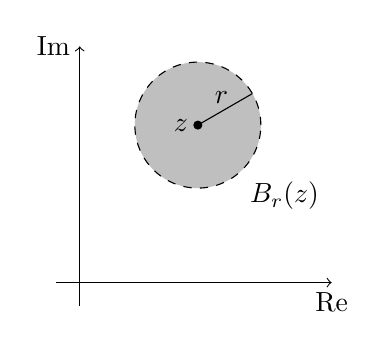
\begin{tikzpicture}
\draw [->] (-0.3,0) -- (3.2,0) node[below] {Re};
\draw [->] (0,-0.3) -- (0,3) node[left] {Im};
\draw[fill=lightgray,dashed] (1.5,2) circle (0.8) node[left] {$z$};
\draw (1.8,2.35) node {$r$};
\draw[fill] (1.5,2) circle (0.05);
\draw (1.5,2) edge +(0.8*cos 30,0.8*sin 30);
\draw (3.3,2.7) node {$\C$};
\draw (2.6,1.1) node {$B_r(z)$};
\end{tikzpicture}
\end{center}

\v

Define $\mathcal{O}_\C$ implicitly by:
\bse
U\in \mathcal{O}_\C\ :\Leftrightarrow\ \forall \, z \in U : \exists \, r>0 : B_r(z)\se U
\ese

\v

Then, the pair $(\C,\mathcal{O}_\C)$ is a topological space. In fact, we have:
\bse
(\C,\mathcal{O}_\C) \cong_\mathrm{top} (\R^2,\mathcal{O}_\mathrm{std})
\ese

We can then equip $\C^4$ with the product topology so that we can finally define:
\bse
\mathcal{O} \coloneqq (\mathcal{O}_\C)|_{\SL(2,\C)}
\ese

so that the pair $(\SL(2,\C),\mathcal{O})$ is a topological space. In fact, it is a connected topological space, and
we will need this property later on.

\subsubsection*{$\SL(2,\C)$ As A Topological Manifold}

Recall that a topological space $(M,\mathcal{O})$ is a complex topological manifold if each point $p\in M$ has an
open neighbourhood $U(p)$ which is homeomorphic to an open subset of $\C^d$. Equivalently, there must exist a
$\mathcal{C}^0$-atlas, i.e.\ a collection $\mathscr{A}$ of charts $(U_\alpha,x_\alpha)$, where the $U_\alpha$ are
open and cover $M$ and each $x$ is a homeomorphism onto a subset of $\C^d$. In our case of $\SL(2,\C)$ we will map it
locally to $\C^3$ because as we said in the beginning of this section, $\SL(2,\C)$ (as a set) is a subset of $\C^4
\coloneqq \C\times\C\times\C\times\C$ due to the constraint $ad-bc = 1$ that removes one degree of freedom. This is
why $\C^3$ suffices and we do not use $\C^4$. \v

In general (but not in our case of $\SL(2,\C)$) nothing stops us from using just one chart $(U,x)$ and cover the
whole topological space. However, as we will see, here we need two charts to cover the whole $\SL(2,\C)$ (in the same
manner that a sphere cannot be covered with just one chart). \v

Let $U$ be the set:
\bse
U \coloneqq \biggl\{ \biggl( \begin{matrix} a & b \\ c & d \end{matrix}\biggr) \in \SL(2,\C) \ \Big| \ a \neq 0 \biggr\}
\ese

and define the map:
\bi{rrCl}
x \cl & U & \to & x(U) \se \C^*\times\C\times \C\\[5pt]
& \biggl( \begin{matrix} a & b \\ c & d \end{matrix}\biggr) & \mapsto & (a,b,c)
\ei

where $\C^*=\C\setminus\{0\}$. \v

Notice that given the mapping $(a,b,c)$ one can reconstruct $d$ from the constraint on the degree of freedom
$d=\frac{1+bc}{a}$, hence, the mapping to $\C^3$. \v

With a little more work on this direction, one can show that $U$ is an open subset of $(\SL(2,\C),\mathcal{O})$ and
$x$ is a homeomorphism with inverse:
\bi{rrCl}
x^{-1} \cl & x(U) & \to & U\\
& (a,b,c)& \mapsto & \biggl( \begin{matrix} a & b \\ c & \frac{1+bc}{a} \end{matrix}\biggr)
\ei

This is the reason why we excluded the case $a=0$ when we defined the set $U$ of the chart $(U,x)$, since if we
hadn't, we wouldn't be able to divide with $a$ and the map $x$ wouldn't have an inverse. \v

However, this makes the chart $(U,x)$ to not cover the whole $\SL(2,\C)$ since $U$ as a set takes care only the
elements of $\SL(2,\C)$ with $a \neq 0$. Hence, we need at least one more chart. We thus define the set:
\bse
V \coloneqq \biggl\{ \biggl( \begin{matrix} a & b \\ c & d \end{matrix}\biggr) \in \SL(2,\C) \ \Big| \ b \neq 0 \biggr\}
\ese

and the map:
\bi{rrCl}
y \cl & V & \to & x(V) \se \C\times \C^*\times \C\\[5pt]
& \biggl( \begin{matrix} a & b \\ c & d \end{matrix}\biggr) & \mapsto & (a,b,d)
\ei

\v

Similarly to the above, $V$ is open and $y$ is a homeomorphism with inverse:
\bi{rrCl}
y^{-1} \cl & x(V) & \to & V\\[5pt]
& (a,b,d)& \mapsto & \biggl( \begin{matrix} a & b \\ \frac{ad-1}{b} & d \end{matrix}\biggr)
\ei

\v

An element of $\SL(2,\C)$ cannot have both $a$ and $b$ equal to zero, for otherwise $ad-bc=0\neq 1$. Hence
$\mathscr{A}_{\mathrm{top}} \coloneqq \{(U,x),(V,y)\}$ is an atlas, and we showed that $x$ and $y$ are homeomorphisms
Hence, continuous and invertible. Since every atlas is automatically a $\mathcal{C}^0$-atlas, the triple $(\SL(2,\C),
\mathcal{O},\mathscr{A}_{\mathrm{top}})$ is a 3-dimensional, complex, topological manifold.

\subsubsection*{$\SL(2,\C)$ As A Complex Differentiable Manifold}

Recall that to obtain a $\mathcal{C}^1$-differentiable manifold from a topological manifold with atlas $\mathscr{A}$,
we have to check that every transition map between charts in $\mathscr{A}$ is differentiable in the usual sense.
Remember this picture:

\vspace{-8pt}

\bse
\begin{tikzcd}
& U\cap V \se \SL(2,\C) \ar[ldd,"x"'] \ar[rdd,"y"]&\\
&&&\\
x(U\cap V) \se \C^3 \ar[rr,"y\circ x^{-1}"']& & y(U\cap V)\se \C^3
\end{tikzcd}
\ese

\vspace{15pt}

In our case, we have the atlas $\mathscr{A}_{\mathrm{top}} \coloneqq \{(U,x),(V,y)\}$. We evaluate:
\bse
(y\circ x^{-1})(a,b,c) = y (\biggl(\begin{matrix} a & b \\ c & \frac{1+bc}{a} \end{matrix}\biggr) ) =
(a,b,\tfrac{1+bc}{a})
\ese

Hence, we have the transition map:
\bi{rrCl}
y\circ x^{-1} \cl & x(U\cap V) & \to & y(U\cap V)\\[5pt]
& (a,b,c) & \mapsto & ( a,b,\tfrac{1+bc}{a})
\ei

Similarly, we have :
\bse
(x\circ y^{-1})(a,b,d) = y (\biggl( \begin{matrix} a & b \\ \frac{ad-1}{b} & d \end{matrix}\biggr) ) =
(a,b,\tfrac{ad-1}{b})
\ese

\v

Hence, the other transition map is :
\bi{rrCl}
x\circ y^{-1} \cl & y(U\cap V) & \to & x(U\cap V)\\[5pt]
& (a,b,c) & \mapsto & ( a,b,\tfrac{ad-1}{b})
\ei

\v

Since $a\neq 0$ and $b\neq 0$, the transition maps are complex differentiable. \v

Therefore, the atlas $\mathscr{A}_{\mathrm{top}}$ is a differentiable atlas. By defining $\mathscr{A}$ to be the
maximal differentiable atlas containing $\mathscr{A}_{\mathrm{top}}$, we have that $(\SL(2,\C),\mathcal{O},
\mathscr{A})$ is a 3-dimensional, complex differentiable manifold.